\documentclass[10pt,twoside,a4paper,fleqn]{report}

\usepackage{braket}
\usepackage{graphicx}
\usepackage{parskip}
\usepackage{amssymb}
\usepackage{mathbbol}
\usepackage{enumerate}
\usepackage{ragged2e}
\usepackage{eurosym}
\usepackage{amsmath}
\usepackage{array}
\usepackage{float}

% Defining some new mathematics commands
\newcommand*{\colvec}[1]{\begin{pmatrix}#1\end{pmatrix}}
\newcommand*{\0}{$\ket{0}$}
\newcommand*{\1}{$\ket{1}$}
\newcommand*{\Title}{A very long table heading}%
\newcommand*{\TitleInParbox}{\parbox[c]{0.3\linewidth}{\Title}}%
\usepackage{array}
\newcolumntype{L}[1]{>{\raggedright\let\newline\\\arraybackslash\hspace{0pt}}m{#1}}
\newcolumntype{C}[1]{>{\centering\let\newline\\\arraybackslash\hspace{0pt}}m{#1}}
\newcolumntype{R}[1]{>{\raggedleft\let\newline\\\arraybackslash\hspace{0pt}}m{#1}}


\usepackage[english,bt]{ethidsc} % Special IDSC styles and commands      	
\usepackage{apacite}
								 % {german}/english: language of headings, etc.
								 % {st}/bt/mt: {semester}/bachelor/master thesis
							
% Page header (don't change)____________________________________________________
\setlength{\parindent}{0em}                 % Disable parindent
\rhead[\nouppercase{\rightmark}]{\thepage}  % Special headings
\lhead[\thepage]{\nouppercase{\leftmark}}   % Special headings
\cfoot{}                                    % Special headings


% Title page (please fill in)___________________________________________________
\title{Quantum-enhanced machine learning:
Implementing a quantum k-nearest neighbour algorithm}


\studentA{Mark Fingerhuth}
\ethidA{I6082973}
\semesterA{5}
\emailA{m.fingerhuth@student.maastrichtuniversity.nl}

\supervision{Prof. Francesco Petruccione\\ Dr. Fabrice Birembaut}
\date{January 2017}

%\identification{} 		% Project identifier

%\infopage %includes the last page
%\declaration

% Begin document________________________________________________________________
\begin{document}

\maketitle 							% Create title page


% Preamble______________________________________________________________________

\pagenumbering{roman} 				% Begin roman page numbering (i,ii,...)

%---------------------------------------------------------------------------
% Preface

\chapter*{Preface}

Blah blah \dots

 \cleardoublepage

%---------------------------------------------------------------------------
% Table of contents

 \setcounter{tocdepth}{2}
 \tableofcontents

 \cleardoublepage

%---------------------------------------------------------------------------
% Abstract

\chapter*{Abstract}
 \addcontentsline{toc}{chapter}{Abstract}

NEEDS MODIFICATION!

Quantum machine learning, the intersection of quantum computation and classical machine learning,
bears the potential to provide more efficient ways to deal with big data through the use of quantum
superpositions, entanglement and the resulting quantum parallelism. The proposed research will
attempt to implement and simulate two quantum machine learning routines and use them to solve
small machine learning problems. That will establish one of the earliest proof-of-concept studies in
the field and demonstrate that quantum machine learning is already implementable on small-scale
quantum computers. This is vital to show that an extrapolation to larger quantum computing devices
will indeed lead to vast speed-ups of current machine learning algorithms.

 \cleardoublepage

%---------------------------------------------------------------------------
% Symbols

\chapter*{Nomenclature}\label{chap:symbole}
 \addcontentsline{toc}{chapter}{Nomenclature}

\section*{Symbols}
\begin{tabbing}
 \hspace*{1.6cm} \= \hspace*{8cm} \= \kill
 $\otimes$ \> Tensor product \\[0.5ex]
 $i$ \> Imaginary unit \> $i=\sqrt{-1}$ \\[0.5ex]
 $\dagger$ \> Hermitian conjugate \> Complex conjugate transpose \\[0.5ex]
 $!$ \> Factorial \> e.g. 3! = 3*2*1 \\[0.5ex]
\end{tabbing}

\section*{Indicies}
\begin{tabbing}
 \hspace*{1.6cm}  \= \kill
 a \> Ambient \\[0.5ex]
 air \> Air
\end{tabbing}

\section*{Acronyms and Abbreviations}
\begin{tabbing}
 \hspace*{1.6cm}  \= \kill
 QML \> Quantum machine learning \\[0.5ex]
 QC \> Quantum computer \\[0.5ex]
 Prob \> Probability \\[0.5ex]
 PM \> Post-measurement \\[0.5ex]
 HD \> Hamming distance \\[0.5ex]
 CM \> Conditional measurement \\[0.5ex]
 CNOT \> Controlled NOT gate \\[0.5ex]
 CCNOT \> Controlled controlled NOT gate (Toffoli gate) \\[0.5ex]
 CU \> Controlled U gate (where U can be any unitary quantum gate) \\[0.5ex]
\end{tabbing}

 \cleardoublepage

%---------------------------------------------------------------------------


% Chapters______________________________________________________________________

\pagestyle{fancy}               	% Fancy headings
\pagenumbering{arabic}				% Begin arabic page numbering (1,2,...)

\chapter{Introduction}\label{sec:introduction}

The ability to recognise familiar faces, to understand spoken language and to distinguish types of vegetables comes naturally to humans, although these processes of pattern recognition and classification are inherently complex. Machine learning (ML), a subdiscipline of artificial intelligence, is concerned with the development of algorithms that perform these types of tasks, thus enabling computers to find and recognise patterns in data and classify unknown inputs based on previous training data. Such algorithms make the core of e.g. human speech recognition and recommendation engines as used by Amazon \cite{graves2013speech,linden2003amazon}.
% and algorithms that can predict heart disease from real-time electrocardiograms \citep{acharya2015integrated, pazzani2007content}.

According to \citeA{bigdata}, approximately 2.5 quintillions (${10}^{18}$) bytes of digital data are created every day. This growing number implies that many areas dealing with data will eventually require advanced algorithms that can make sense of data content, retrieve patterns and reveal correlations. However, most ML algorithms involve the execution of computationally expensive operations and doing so on large data sets inevitably takes a lot of time \cite{bekkerman2011scaling}. Thus, it becomes increasingly important to find efficient ways of dealing with big data.
%and/or reduce the computational complexity of the algorithms.

A promising solution is the use of quantum computation which has been researched intensively in the last few decades. Quantum computers (QCs) use quantum mechanical systems and their unique properties to manipulate and process information in ways that are impossible for classical computers. Analogous to a classical computer manipulating bits, a quantum computer makes use of so-called quantum bits (qubits). Bits and qubits are both binary entities meaning they can only take the values 0 and 1. However, a non-probabilistic classical bit can only take one of these values at a time whereas a qubit can also be found in a linear superposition of the two states.

%\begin{equation}
%\label{equ: simplequbit}
%\ket{q} = \alpha \ket{0} + \beta \ket{1}
%\end{equation}
%where $\alpha$ and $\beta$ are complex numbers and often referred to as amplitudes. When measuring qubit $\ket{q}$ it will take the value \0 with a probability of ${|\alpha|}^{2}$ and \1 with a probability of ${|\beta|}^{2}$. Since the total probability has to sum to unity, the normalization condition ${|\alpha|}^{2} + {|\beta|}^{2} =  1$ must be satisfied at all times.

This property gives rise to quantum parallelism, which enables the execution of certain operations on many quantum states at the same time. Despite this advantage, the difficulty in quantum computation lies in the retrieval of the computed solution since a measurement of a qubit collapses it into a single classical bit and thereby destroys information about its previous superposition. Several quantum algorithms have been proposed that provide exponential speed-ups when compared to their classical counterparts with Shor's prime factorization algorithm being the most famous \cite{shor1994}.
%As another example, Grover's quantum database search algorithm enables finding a single element in a list of $N$ elements within roughly $\sqrt{N}$ quantum mechanical steps instead of $N$ classical steps \citep{grover}.
Thus, quantum computation has the potential to improve computational power, speed up the processing of big data and possibly solve certain problems that are practically unsolvable on classical computers e.g. computationally-exhaustive optimisation problems such as the well-known travelling salesman problem with more than 1000 cities \cite{kieu2006quantum}.

%for the QML toolbox to be complete a quantum algorithm to solve systems of linear equations is needed since most ML algorithms rely on solving those.

Considering these advantages, the combination of quantum computation and classical ML into the new field of quantum machine learning (QML) seems almost natural. More specifically, one speaks of quantum-enhanced machine learning when quantum computation is used to improve classical ML algorithms. Yet, both fields are mutually beneficial to each other since classical ML can also be used to improve aspects of quantum computation. For example, \citeA{las2016genetic} showed that a classical genetic algorithm can be used to reduce the experimental error in quantum logic gates. However, this thesis will only focus on the field of quantum-enhanced machine learning.

%There are currently two main ideas on how to merge quantum computation with ML, namely a) running the classical algorithm on a classical computer and outsourcing only the computationally intensive task to a QC or b) executing the quantum version of the entire algorithm on a QC. Current QML research mostly focusses on the latter approach by developing quantum algorithms that tap into the full potential of quantum parallelism.

\section{Motivation}
\label{sec:motivation}

Classical ML is a very practical topic since it can be directly tested, verified and implemented on any commercial classical computer. So far, QML has been of almost entirely theoretical nature since the required computational resources are not yet in place. To yield reliable solutions QML algorithms often require a huge number of error-correcting qubits and some quantum data storage such as the proposed quantum random access memory (qRAM) \cite{qRAM}. However, to date the maximum number of e.g. superconducting qubits reportedly used for calculation is nine, the D-Wave II quantum annealing device delivers 1152 qubits but can only solve a narrow class of problems, and a qRAM has not been developed yet \cite{hydrogensimulation, dwave2}. Furthermore, qubit error-correction is still a very active research field, and most of the described preliminary QCs deal with non-error-corrected qubits with short lifetimes and are, thus, impractical for large QML implementations.

Until now there have been only a few experimental verifications of QML algorithms that establish proof-of-principle. \citeA{Li2015} successfully distinguished handwritten digits using a quantum support vector machine on a four-qubit nuclear magnetic resonance test bench. In addition, \citeA{Cai2015} were first to experimentally demonstrate quantum machine learning on a photonic QC and showed that the distance between two vectors and their inner product can indeed be computed quantum mechanically. Lastly, \citeA{Riste2015} solved a learning parity problem with five superconducting qubits and found that a quantum advantage can already be observed in non-error-corrected systems.

%Consequently,
Considering the gap between the number of proposed QML algorithms and the few experimental realisations, it becomes important to find QML problems which can already be implemented on small-scale QCs. Hence, the purpose of this research is to provide proof-of-principle implementations and simulations of selected QML algorithms on small datasets. For this purpose, the $k$-nearest neighbour algorithm, one of the simplest ML algorithms, was chosen as a good minimal example for implementation and quantum simulation. This is a necessary step in the attempt to shift QML from a purely theoretical research area to a more applied field such as classical ML.

\section{Research question}
\label{sec:researchquestion}


%Don't know where this should go!

%Matthias Troyer citation for this part:

%Finding optimal ways of compiling a given quantum algorithm as well as designing a high-level programming language or environment similar to that of classical computer code editors is called \emph{quantum software engineering}.

In light of the theoretical nature of current QML research and the small number of experimental realisations, this research will address the following question:

%NARROW DOWN THE RESEARCH QUESTION!
\centering\textbf{How can a k-nearest neighbour quantum machine learning algorithm be implemented on small-scale quantum computers?}

%Alternatives:
%Is it possible to experimentally demonstrate that two QML algorithms proposed by \cite{Schuld2014, Schuld2016} can already solve a small ML problem using classical simulation or IBMs quantum processor?
%Is it possible to already implement and solve a small ML problem on IBMs publicly available quantum computer?

\justify
The following sections will introduce the necessary theoretical foundations, and the tools used to answer this research question. 

\cleardoublepage
\chapter{Theoretical Foundations and Methods}\label{sec:theoryandmethods}

\section{Quantum Bits}
\label{subsec:qubits}

\subsection{Single Qubit Systems}
\label{subsubsec:qubits}
%Classical computers manipulate bits and the quantum equivalent is called a quantum bit, often abbreviated as qubit.
Classical computers manipulate bits, whereas quantum computer's most fundamental unit is called a quantum bit, often abbreviated as qubit. Bits as well as qubits are binary entities, meaning they can only take the values 0 and 1. A classical non-probabilistic bit can only be in one of the two possible states at once. In contrast, qubits obey the laws of quantum mechanics, which gives rise to the powerful property that - besides being a definite 0 or 1 - they can also be in a superposition of the two states. Mathematically this is expressed as a linear combination of the states 0 and 1:
\begin{equation}
\label{equ: simplequbit}
\ket{\psi} = \alpha \ket{0} + \beta \ket{1}
\end{equation}
where $\alpha$ and $\beta$ are complex coefficients ($\alpha, \beta \in \mathbb{C}$) and are often referred to as phase factors or amplitudes. \0 is the Dirac notation for the qubit being in state 0 and it represents a two-dimensional vector in a complex 2-D vector space (called Hilbert space $\mathcal{H}_{2}$). \0 and \1 are the computational basis states and they constitute an orthonormal basis of $\mathcal{H}_{2}$. For the sake of clarity, \0 and \1 can be thought of as the 2-D vectors shown below.
\begin{equation}
\label{equ: 0and1kets}
\ket{0} =  \colvec{1\\0} \quad \quad \ket{1} = \colvec{0\\1}
\end{equation}

Subbing these vectors into Equ.~\ref{equ: simplequbit} yields the vector representation of $\ket{\psi}$:
\begin{equation}
\label{equ: simplequbitvector}
\ket{\psi} = \alpha \colvec{1\\0} + \beta \colvec{0\\1} = \colvec{\alpha\\\beta}
\end{equation}

However, even though a qubit can be in a superposition of \0 and \1, when measured it will take the value \0 with a probability of
\begin{equation}
\label{equ:bornrule0}
Prob(\ket{0}) = {|\alpha|}^{2}
\end{equation}
and \1 with a probability of 
\begin{equation}
\label{equ:bornrule1}
Prob(\ket{1}) = {|\beta|}^{2}
\end{equation}

The fact that the probability of measuring a particular state is equal the absolute value squared of the respective amplitude is called Born's rule (citation). Since the total probability of measuring any value has to be 1, the following normalization condition must be satisfied:
\begin{equation}
\label{equ: normalization}
{|\alpha|}^{2} + {|\beta|}^{2} =  1
\end{equation}
Therefore, a qubit is inherently probabilistic but when measured it collapses into a single classical bit (0 or 1). It follows that a measurement destroys information about the superposition of the qubit (the values of $\alpha$ and $\beta$). This constitutes one of the main difficulties when designing quantum algorithms since only limited information can be obtained about the final states of the qubits in the quantum computer.

Similar to logic gates in a classical computer, a QC manipulates qubit by means of quantum logic gates which will be introduced in detail in Section~\ref{subsec:quantumlogicgates}. Generally, an arbitrary quantum logic gate U acting on a single qubit state is a linear transformation given by a 2x2 matrix whose action on $\ket{\psi}$ is defined as:

\begin{equation}
\label{equ:unitarytransformation}
U \ket{\psi} = \begin{pmatrix}
 a & b \\ 
 c & d
 \end{pmatrix} \colvec{\alpha\\\beta} = \colvec{a*\alpha+b*\beta\\c*\alpha+d*\beta}
\end{equation}

Matrix $U$ must be unitary which means that a) its determinant is equal to unity and b) its Hermitian conjugate $U^\dagger$ must be equal to its inverse. These properties are expressed in Equ.~\ref{equ:unitarydef1} and ~\ref{equ:unitarydef2} below. All quantum logic gates must be unitary since this preserves the normalization of the qubit state it is acting on.

\begin{align}
\label{equ:unitarydef1}
a)& \mid det(U) \mid = 1 \\ 
\label{equ:unitarydef2}
b)& \quad UU^\dagger = U^\dagger U = \mathbb{1} = UU^{-1} = U^{-1}U
\end{align} 

Using spherical polar coordinates, a single qubit can be visualized on the so-called Bloch sphere by parameterising $\alpha$ and $\beta$ in Equ.~\ref{equ: simplequbit} as follows:

\begin{equation}
\label{equ: blochqubit}
\ket{q} = \cos\frac{\theta}{2} \ket{0} + e^{i \phi} \sin\frac{\theta}{2} \ket{1}
\end{equation}

The Bloch sphere has a radius of 1 and is therefore a unit sphere. The \0 qubit state is defined to lie along the positive z-axis ($\hat{z}$) and the \1 state is defined to lie along the negative z-axis ($-\hat{z}$) as labelled in Fig.~\ref{fig:blochsphere}. At this point, it is important to note that these two states are mutually orthogonal in $\mathcal{H}_{2}$ even though they are not orthogonal on the Bloch sphere. 

Qubit states on the Bloch equator such as the $\hat{x}$ and $\hat{y}$ coordinate axes represent equal superpositions where \0 and \1 both have measurement probabilities equal to $0.5$. The $\hat{x}$-axis for example represents the equal superposition $\ket{q} = \frac{1}{\sqrt{2}} \ket{0} + \frac{1}{\sqrt{2}} \ket{1}$. As illustrated in Fig.~\ref{fig:blochsphere} any arbitrary 2-D qubit state $\ket{\psi}$ can be decomposed into the polar angles $\theta$ and $\phi$ and visualized as a vector on the Bloch sphere. Such an object is called the Bloch vector of the qubit state $\ket{\psi}$. The Bloch sphere will be the main visualization tool for qubit manipulations in this thesis.

\begin{figure}[!ht]
       \centering
       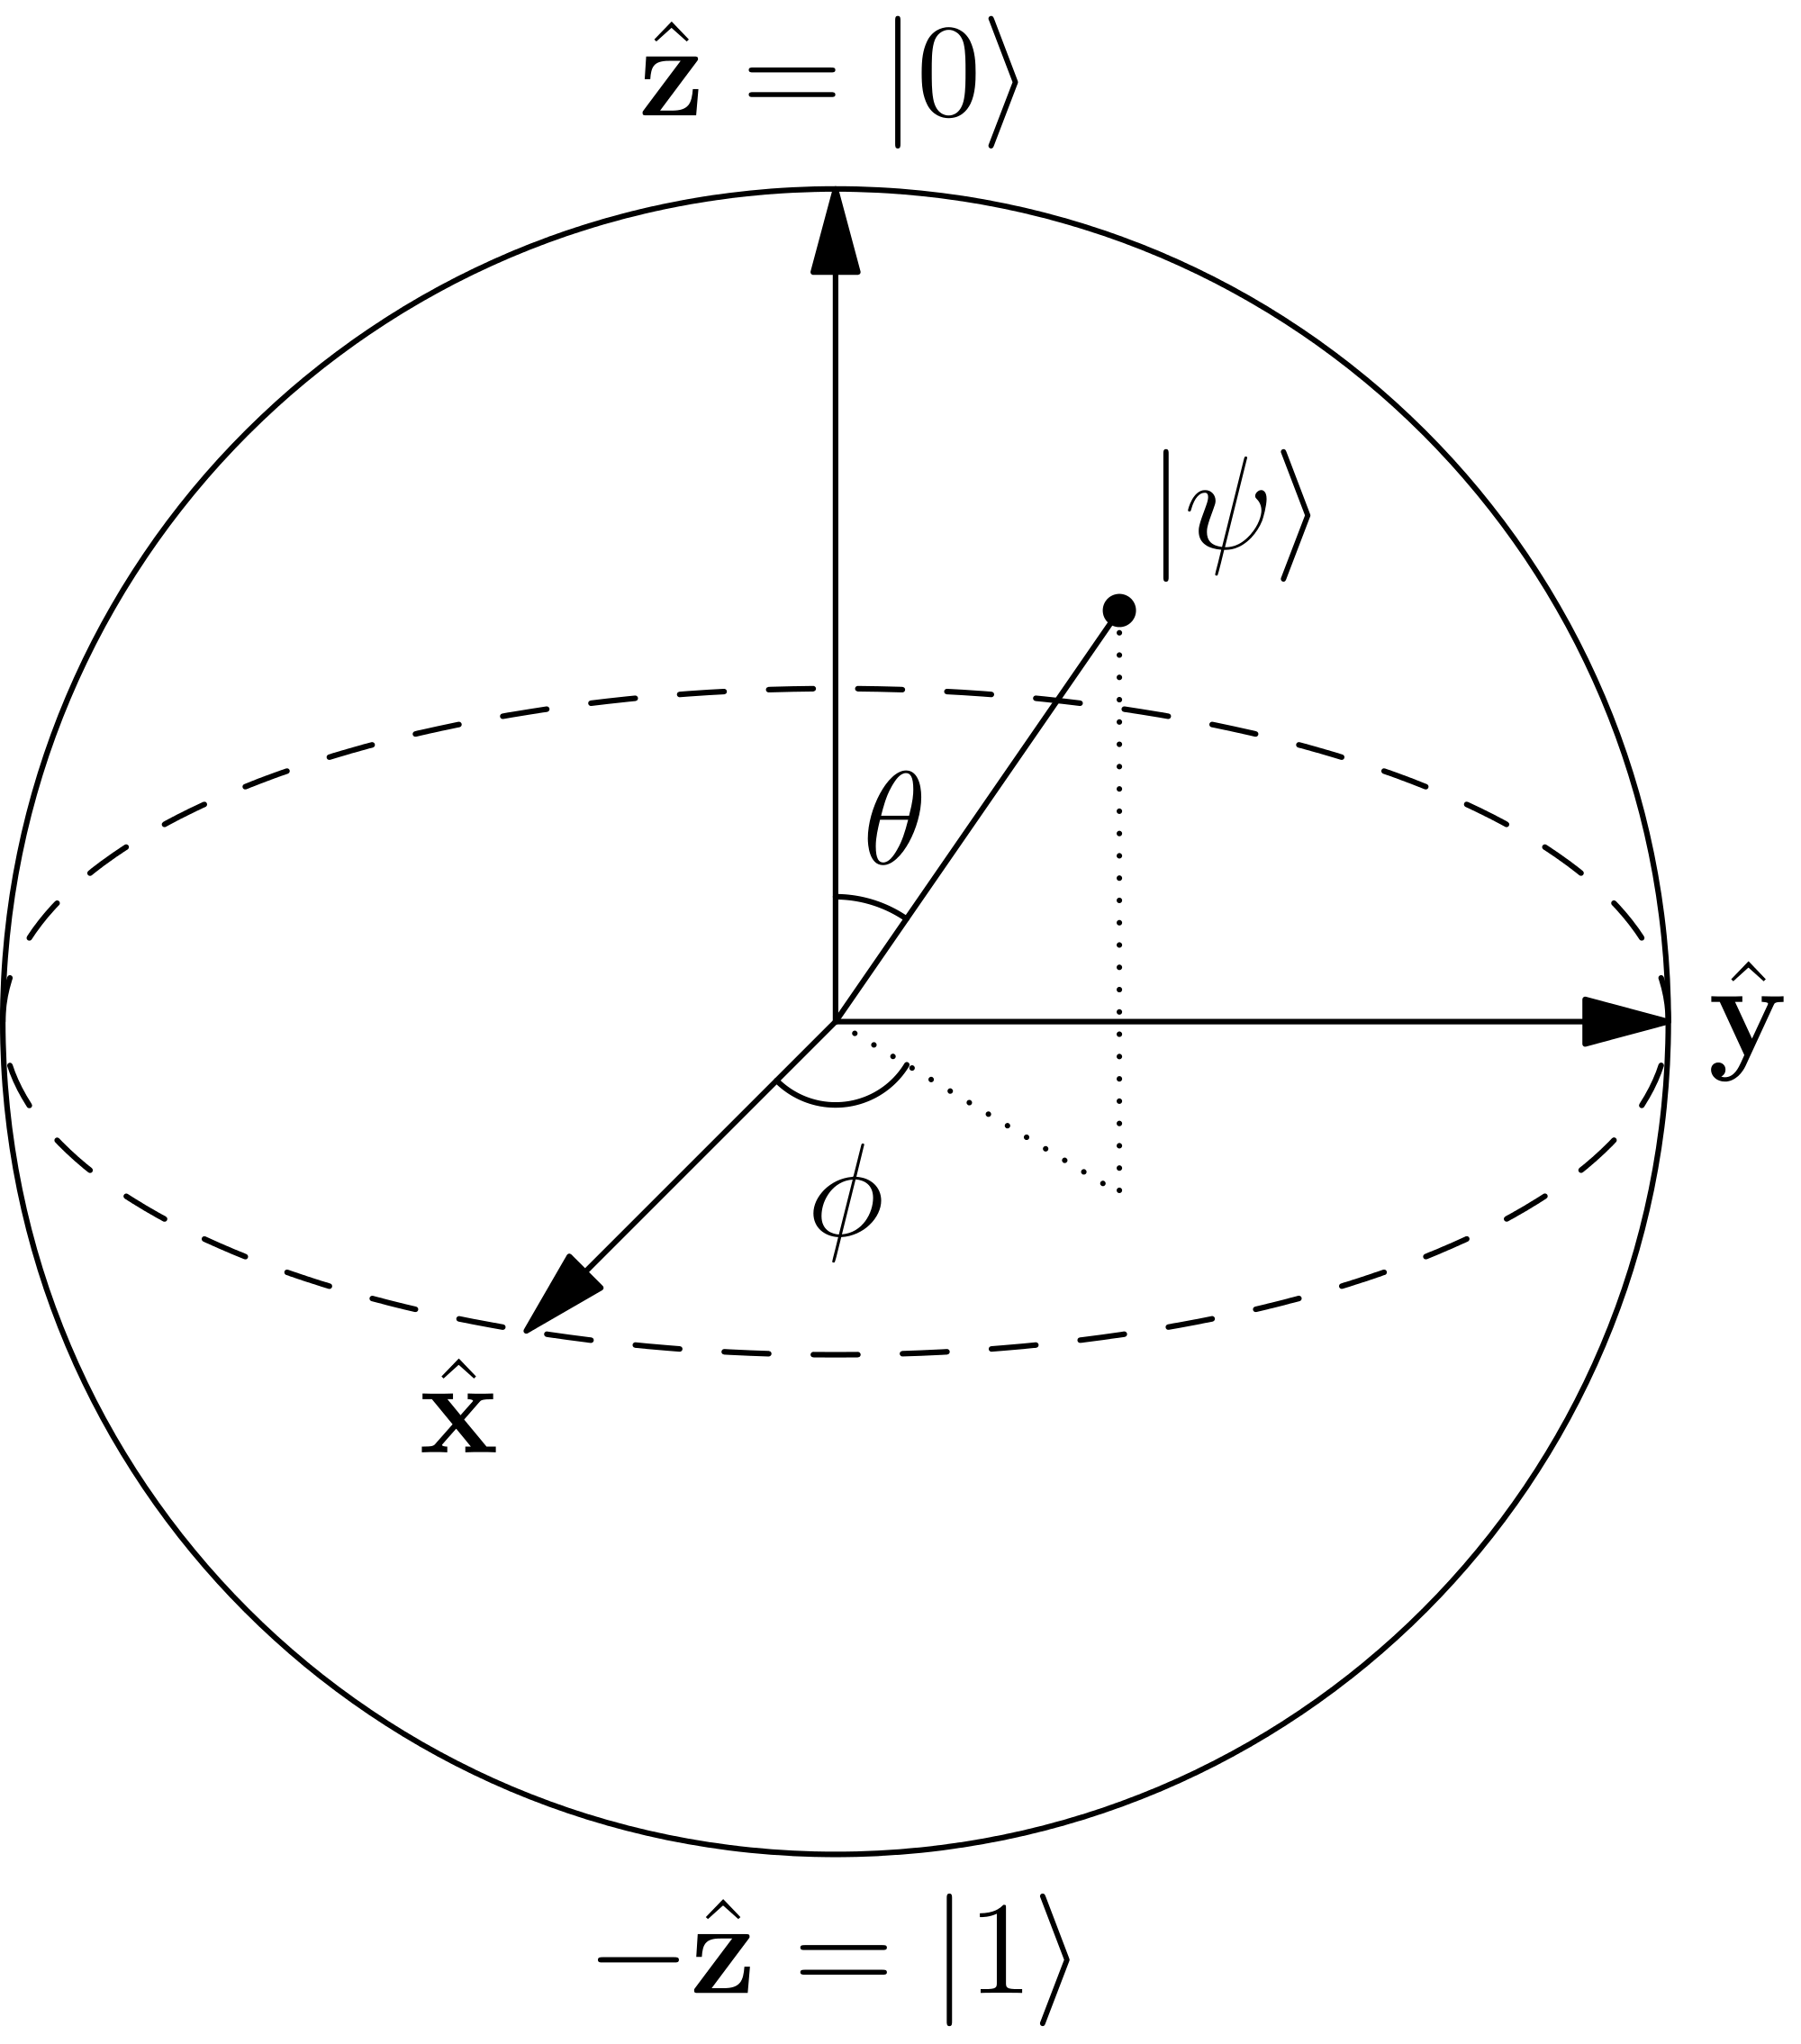
\includegraphics[scale=0.07]{img/blochsphere.png}
       \caption{\label{fig:blochsphere} An arbitrary two-dimensional qubit $\ket{\psi}$ visualized on the Bloch sphere.$^{1}$}
\end{figure}

\footnotetext[1]{Reprinted from Wikipedia, n.d., Retrieved September 7, 2016, from \url{https://en.wikipedia.org/wiki/Bloch_Sphere}. Copyright 2012 by Glosser.ca. Reprinted with permission.}

\subsection{Multiple Qubit Systems}
\label{subsec:multiplequbitsystems}

When moving from single to multi qubit systems a new mathematical tool, the so-called tensor product (symbol $\otimes$), is needed. A tensor product of two qubits is written as:

\begin{equation}
\ket{\psi} \otimes \ket{\psi} = \ket{0} \otimes \ket{0} = \ket{00}
\end{equation}
 
whereby the last expression omits the $\otimes$ symbol which is the shorthand form of a tensor product between two qubits.

In vector notation a tensor product of two vectors (\textcolor{red}{red} and \textcolor{green}{green}) is defined as shown below:

\begin{equation}
\label{equ:tensor2qubits}
\ket{\textcolor{red}{0}\textcolor{green}{0}} = \textcolor{red}{\ket{0}} \otimes \textcolor{green}{\ket{0}} = \textcolor{red}{\colvec{1\\0}} \otimes \textcolor{green}{\colvec{1\\0}} = \colvec{\textcolor{red}{1}*\textcolor{green}{\colvec{1\\0}}\\\textcolor{red}{0}*\textcolor{green}{\colvec{1\\0}}} = \colvec{1\\0\\0\\0}
\end{equation}

The last expression in Equ.~\ref{equ:tensor2qubits} shows that the two-qubit state $\ket{00}$ is no longer two but four-dimensional. Hence, it lives in a four-dimensional Hilbert space $\mathcal{H}_{4}$. A quantum gate acting on multiple qubits can therefore not have the same dimensions as a single-qubit gate (Equ.~\ref{equ:unitarytransformation}) which demands for a new gate formalism for multi qubit systems.

Consider wanting to apply an arbitrary single-qubit gate U (Equ.~\ref{equ:unitarytransformation}) to the first qubit and leaving the second qubit unchanged, essentially applying the identity matrix $\mathbb{1}$ to it. To do this, one defines the tensor product of two matrices as follows,

\begin{equation}
\label{equ:matrixtensorproduct}
\textcolor{red}{U} \otimes \textcolor{green}{\mathbb{1}} =\textcolor{red}{\begin{pmatrix}
 a & b \\ 
 c & d
 \end{pmatrix}} \otimes \textcolor{green}{\begin{pmatrix}
 1 & 0 \\ 
 0 & 1
 \end{pmatrix}} = \begin{pmatrix}
 \textcolor{red}{a}*\textcolor{green}{\begin{pmatrix}
 1 & 0 \\ 
 0 & 1
 \end{pmatrix}} & \textcolor{red}{b}*\textcolor{green}{\begin{pmatrix}
 1 & 0 \\ 
 0 & 1
 \end{pmatrix}} \\ 
 \textcolor{red}{c}*\textcolor{green}{\begin{pmatrix}
 1 & 0 \\ 
 0 & 1
 \end{pmatrix}} & \textcolor{red}{d}*\textcolor{green}{\begin{pmatrix}
 1 & 0 \\ 
 0 & 1
 \end{pmatrix}}
 \end{pmatrix} = \begin{pmatrix}
 a & 0 & b & 0 \\ 
 0 & a & 0 & b \\ 
 c & 0 & d & 0 \\ 
 0 & c & 0 & d 
 \end{pmatrix}
\end{equation}

Thus, the result of the tensor product $U \otimes \mathbb{1}$ is a unitary 4x4 matrix which can now be used to linearly transform the 4x1 vector representing the $\ket{00}$ state in Equ.~\ref{equ:tensor2qubits}:

\begin{equation}
\label{equ:2qubitlineartransform1}
U \otimes \mathbb{1} \ket{00} = \begin{pmatrix}
 a & 0 & b & 0 \\ 
 0 & a & 0 & b \\ 
 c & 0 & d & 0 \\ 
 0 & c & 0 & d 
 \end{pmatrix} \colvec{1\\0\\0\\0} = \colvec{a\\0\\c\\0}
\end{equation}

One can also first perform the single qubit operations on the respective qubits followed by the tensor product of the two resulting vectors:

\begin{equation}
\label{equ:2qubitlineartransform2}
(U \otimes \mathbb{1})(\ket{0} \otimes \ket{0})= U\ket{0} \otimes \mathbb{1}\ket{0} = \begin{pmatrix}
 a & b \\ 
 c & d
 \end{pmatrix} \colvec{1\\0} \otimes \begin{pmatrix}
 1 & 0 \\ 
 0 & 1
 \end{pmatrix} \colvec{1\\0} = \colvec{a\\c} \otimes \colvec{1\\0} = \colvec{a\\0\\c\\0}
\end{equation}

This formalism can be extended to any number of qubits and 

\subsection{Entanglement}
\label{subsec:entanglement}

Introduce entanglement and non-factorising tensor states here!

%%%%% SECTION: Q LOGIC GATES


\section{Quantum Logic Gates}
\label{subsec:quantumlogicgates}
In order to perform quantum computations, tools, analogous to the classical logic gates, are needed for qubit manipulation. Quantum logic gates are square matrices that can be visualized as rotations on the Bloch sphere. The following subsections will introduce the major single and multi qubit logic gates.

\subsection{Single Qubit Gates}
\label{subsubsec:singlequbitgates}

\begin{table}[ht!]
\caption{Table of major single-qubit quantum logic gates.}\vspace{1em}
\label{tab:singlequbitgates}
\begin{tabular}{ C{0.3cm}  C{2cm}  C{1.5cm}  C{1.5cm} C{2.5cm} C{2cm} C{3.5cm}}\hline
Gate & Name & Circuit representation & Matrix & Description & Rotation & Bloch sphere \\ \midrule
$\mathbb{1}$ & Identity & 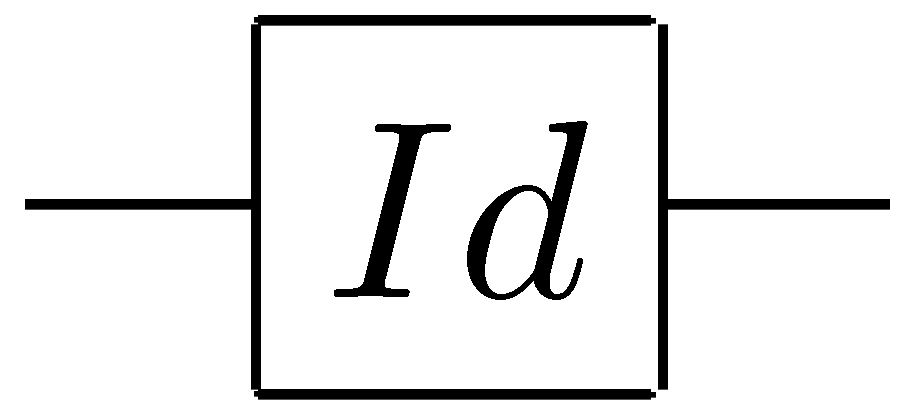
\includegraphics[width=0.1\textwidth]{img/identitycircuit.png} & $\begin{pmatrix}
 1 & 0 \\ 
 0 & 1
 \end{pmatrix}$ & Idle or waiting gate & - & - \\\midrule
X & Qubit flip & 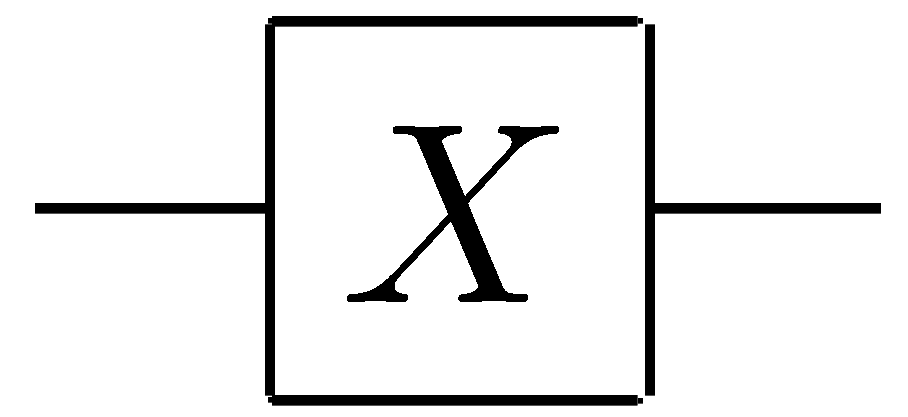
\includegraphics[width=0.1\textwidth]{img/xcircuit.png}  & $\begin{pmatrix}
 0 & 1 \\ 
 1 & 0
 \end{pmatrix}$ & Swaps amplitudes of \0 and \1 & $\pi$ rotation around $\hat{x}$ & 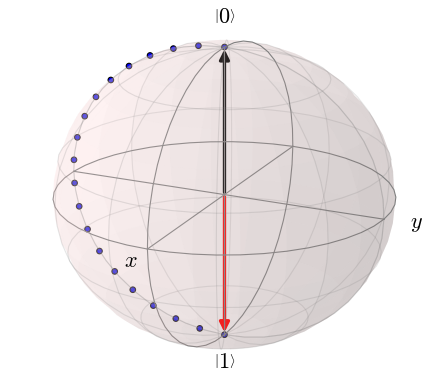
\includegraphics[width=0.2\textwidth]{img/blochxgate.png}\\\midrule
Y & Qubit \& phase flip & 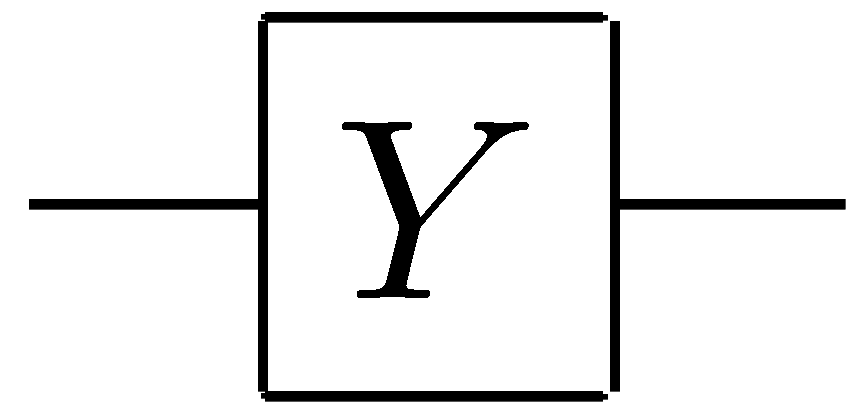
\includegraphics[width=0.1\textwidth]{img/ycircuit.png}  & $\begin{pmatrix}
 0 & -i \\ 
 i & 0
 \end{pmatrix}$ & Swaps amplitudes and introduces phase & $\pi$ rotation around $\hat{y}$ &  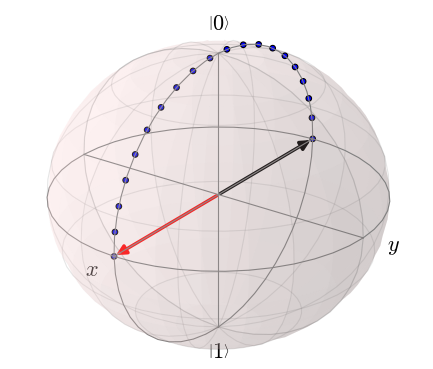
\includegraphics[width=0.2\textwidth]{img/blochygate.png}\\\midrule
Z & Phase flip & 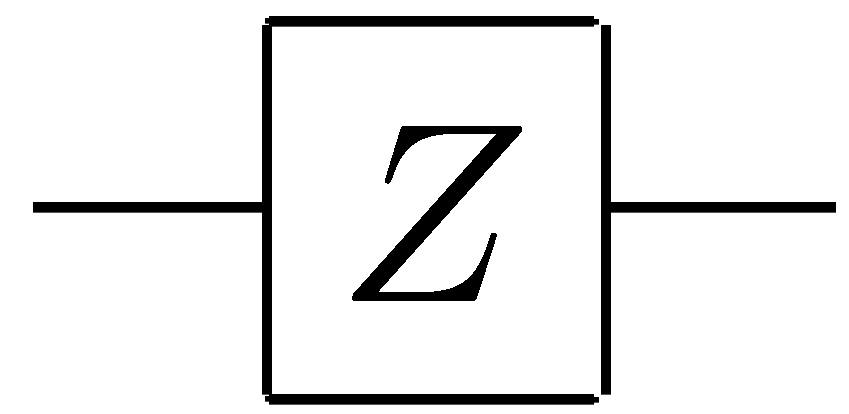
\includegraphics[width=0.1\textwidth]{img/zcircuit.png} & $\begin{pmatrix}
 1 & 0 \\ 
 0 & -1
 \end{pmatrix}$ & Adds a negative sign to the \1 state & $\pi$ rotation around $\hat{z}$ & 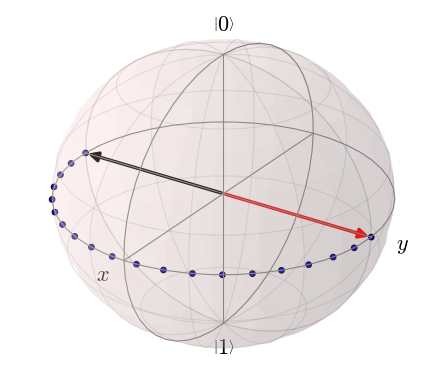
\includegraphics[width=0.2\textwidth]{img/blochzgate.png} \\\midrule 
H & Hadamard & 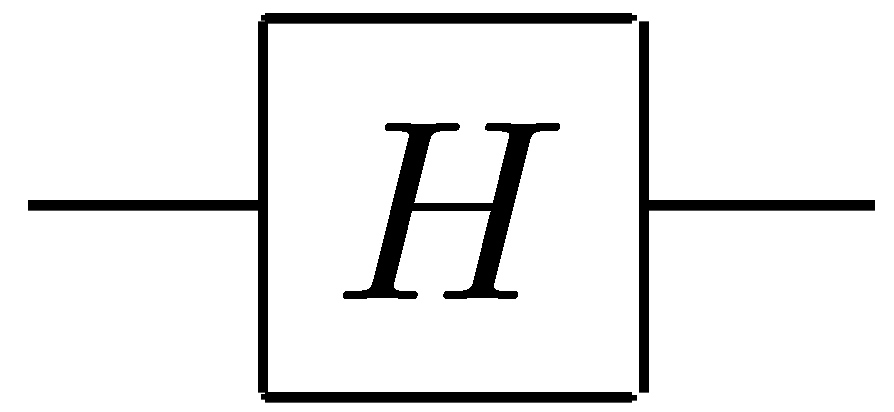
\includegraphics[width=0.1\textwidth]{img/hcircuit.png}  & $\begin{pmatrix}
 \frac{1}{\sqrt{2}} & \frac{1}{\sqrt{2}} \\ 
 \frac{1}{\sqrt{2}} & -\frac{1}{\sqrt{2}}
 \end{pmatrix}$ & Creates equal superpositions & $\frac{\pi}{2}$ rotation around $\hat{y}$ and $\pi$ rotation around $\hat{x}$ & 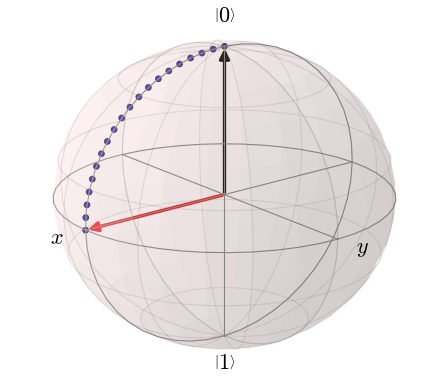
\includegraphics[width=0.2\textwidth]{img/blochhadamard.png}\\\midrule
S & $\frac{\pi}{2}$ rotation gate & 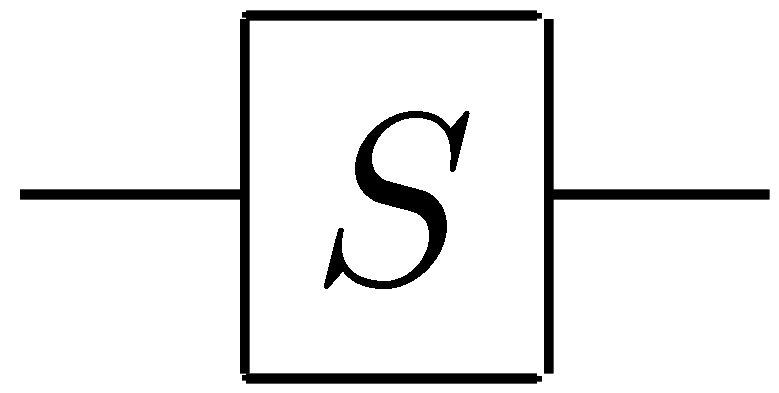
\includegraphics[width=0.1\textwidth]{img/scircuit.png} & $\begin{pmatrix}
 1 & 0 \\ 
 0 & i
 \end{pmatrix}$ & $\sqrt{Z}$ & $\frac{\pi}{2}$ rotation around $\hat{z}$ &  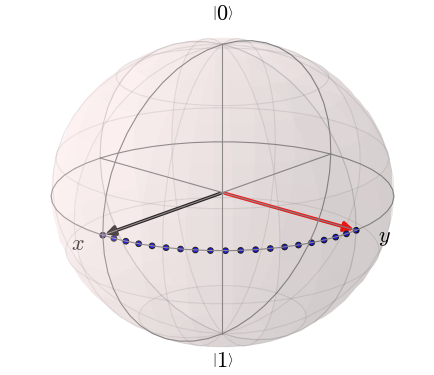
\includegraphics[width=0.2\textwidth]{img/blochsgate.png}\\\midrule
S$^\dagger$ & $-\frac{\pi}{2}$ rotation gate & 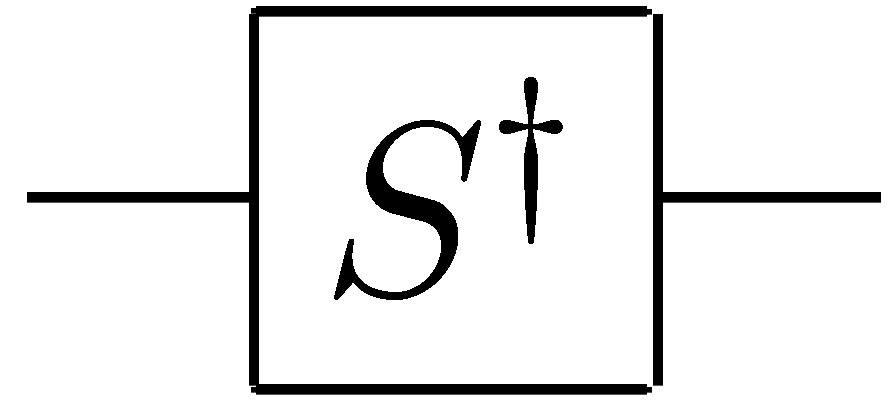
\includegraphics[width=0.1\textwidth]{img/sdcircuit.png} &  $\begin{pmatrix}
 1 & 0 \\ 
 0 & -i
 \end{pmatrix}$ & Adjoint of S & $-\frac{\pi}{2}$ rotation around $\hat{z}$ & \\\midrule
T & $\frac{\pi}{4}$ rotation gate & 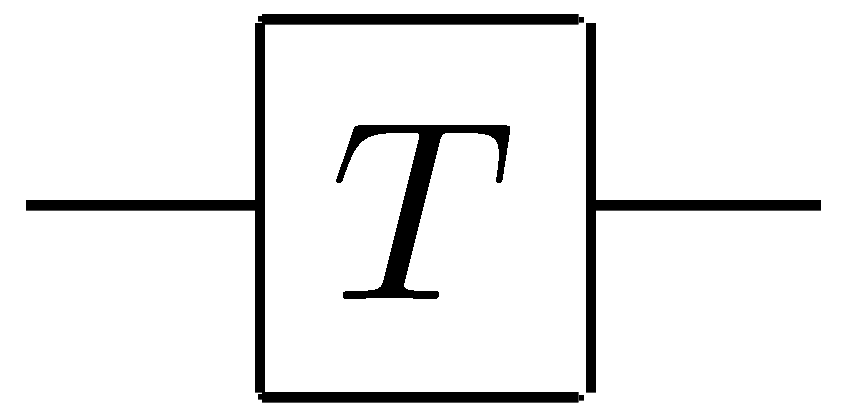
\includegraphics[width=0.1\textwidth]{img/tcircuit.png} & $\begin{pmatrix}
 1 & 0 \\ 
 0 & e^{\frac{i\pi}{4}}
 \end{pmatrix}$ & $\sqrt{S}$ & $\frac{\pi}{4}$ rotation around $\hat{z}$ & 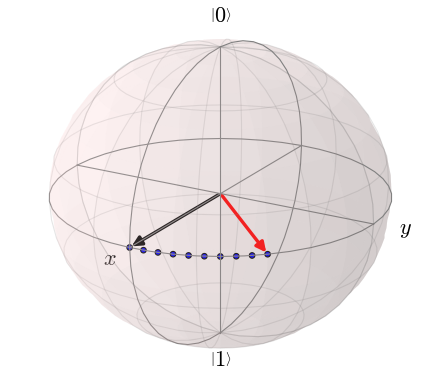
\includegraphics[width=0.2\textwidth]{img/blochtgate.png}\\\midrule
T$^\dagger$ & $-\frac{\pi}{4}$ rotation gate & 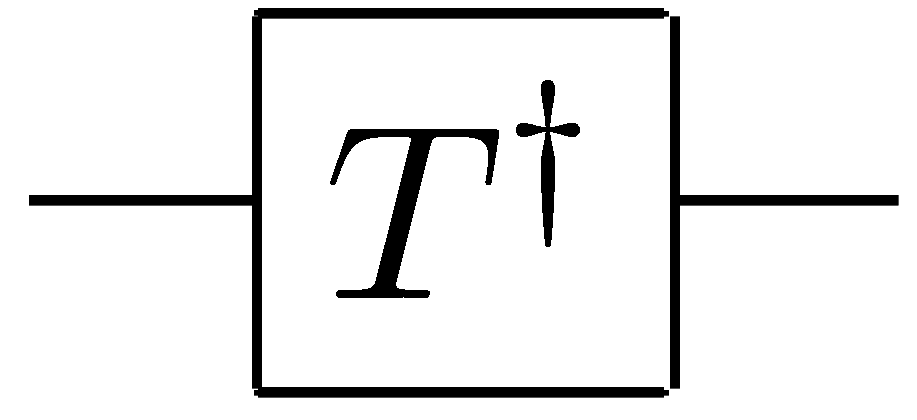
\includegraphics[width=0.1\textwidth]{img/tdcircuit.png} & $\begin{pmatrix}
 1 & 0 \\ 
 0 & e^{-\frac{i\pi}{4}}
 \end{pmatrix}$ & Adjoint of T & $-\frac{\pi}{4}$ rotation around $\hat{z}$ & \\\midrule
ZM & Z-basis measurement & 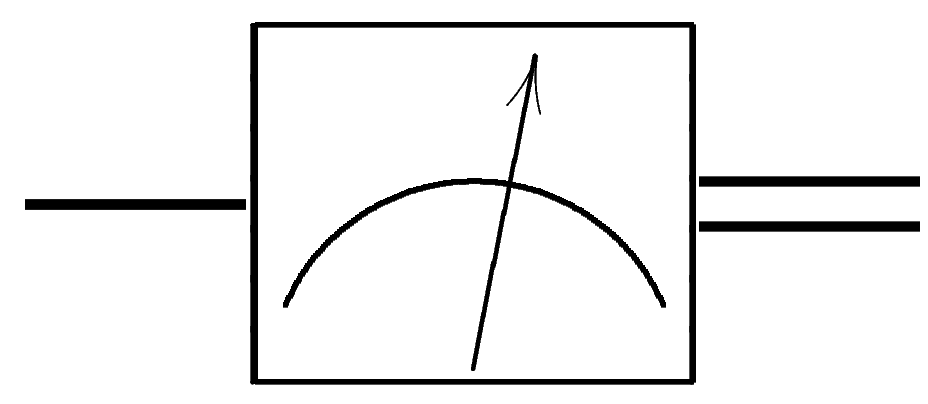
\includegraphics[width=0.1\textwidth]{img/measurecircuit.png} & - & Measurement in standard basis & Collapses the state & - \\
%\midrule
%BM & Bloch measurement & 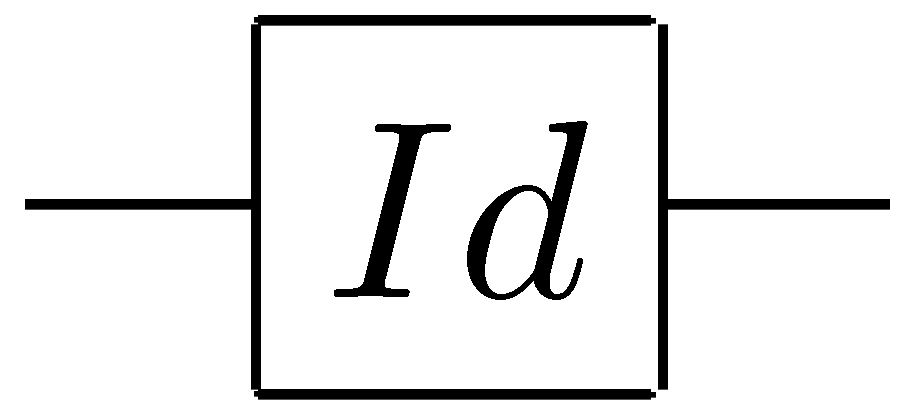
\includegraphics[width=0.1\textwidth]{img/identitycircuit.png} & - & Quantum state tomography & Collapses the state  & -\\
\end{tabular}
\end{table}


%%%%% SUBSECTION: MULTIPLE Q LOGIC GATES


\subsection{Multiple Qubit Gates}
\label{subsubsec:multiqubitgates}

\subsubsection{Controlled NOT Gate}
\label{subsubsubsec:cnotgate}

The most important two-qubit quantum gate is the controlled NOT or CNOT gate given by the following 4x4 matrix:
\begin{equation}
CNOT = \begin{pmatrix}
 \mathbb{1} & 0 \\ 
 0 & X
 \end{pmatrix} = \begin{pmatrix}
 1 & 0 & 0 & 0 \\ 
 0 & 1 & 0 & 0 \\
 0 & 0 & 0 & 1 \\
 0 & 0 & 1 & 0 \\
 \end{pmatrix}
\end{equation}

The CNOT gate takes two qubits, control and target qubit, as input. If and only if the control qubit is in the \1 state, the NOT (X) gate is applied to the target qubit. In equations, the CNOT will always be followed by parantheses containing the control qubit followed by the target qubit (e.g. CNOT(0,1)). The input-output relation for the CNOT gate is given in Table~\ref{tab:cnottruthtable} below.

\begin{table}[ht!]
\begin{center}
\caption{CNOT truth table with first qubit as control, second qubit as target.}\vspace{1ex}
\label{tab:cnottruthtable}
\begin{tabular}{llccc}\hline
Input & Output \\ \hline
00 & 00 \\
01 & 01 \\
10 & 11 \\
11 & 10 \\ \hline
\end{tabular}
\end{center}
\end{table}

To demonstrate the usefulness of the CNOT gate consider starting with two unentangled qubits both in the \0 state,

\begin{equation}
\ket{\phi} = \ket{0} \otimes \ket{0} = \ket{00}
\end{equation}

Applying the H gate onto the first qubit yields the following (still unentangled) state:

\begin{equation}
(H \otimes \mathbb{1}) \ket{\phi} = (H \otimes \mathbb{1}) \ket{00} = \frac{1}{\sqrt{2}} \ket{00} + \frac{1}{\sqrt{2}} \ket{10} 
\end{equation}

Now consider applying the CNOT to this state whereby the control qubit is coloured \textcolor{red}{red} and the target qubit \textcolor{green}{green}.

\begin{equation}
\label{equ:cnotexamples}
CNOT(\textcolor{red}{0},\textcolor{green}{1}) \otimes (\frac{1}{\sqrt{2}} \ket{\textcolor{red}{0}\textcolor{green}{0}} + \frac{1}{\sqrt{2}} \ket{\textcolor{red}{1}\textcolor{green}{0}}) = \frac{1}{\sqrt{2}} \ket{\textcolor{red}{0}\textcolor{green}{0}} + \frac{1}{\sqrt{2}} (\mathbb{1} \otimes X) \ket{\textcolor{red}{1}\textcolor{green}{0}} = \frac{1}{\sqrt{2}} \ket{\textcolor{red}{0}\textcolor{green}{0}} + \frac{1}{\sqrt{2}} \ket{\textcolor{red}{1}\textcolor{green}{1}}
\end{equation}

The last expression in Equ.~\ref{equ:cnotexamples} is one of the famous Bell states which are four maximally entangled states. Thus, this example demonstrates how the CNOT gate is crucial for the generation of entangled states since it applies the X gate to a qubit depending on the state of a second qubit.

\begin{table}[ht!]
\caption{Table of major multi-qubit quantum logic gates.}\vspace{1em}
\label{tab:multiqubitgates}
\begin{tabular}{ c  C{1.8cm}  C{2cm}  c C{3cm}}\hline
Gate & Name & Circuit representation & Matrix & Description \\ \midrule
CNOT & Controlled NOT & 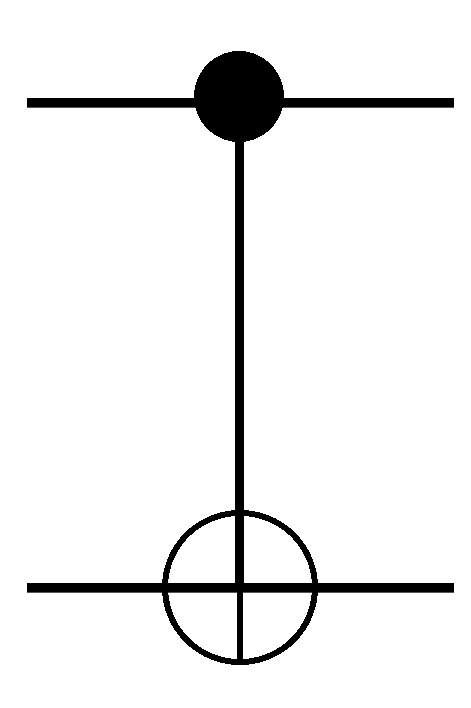
\includegraphics[width=0.1\textwidth]{img/cnotcircuit.png} & $\begin{pmatrix}
 \mathbb{1} & 0 \\ 
 0 & X
 \end{pmatrix} = \begin{pmatrix}
 1 & 0 & 0 & 0 \\ 
 0 & 1 & 0 & 0 \\
 0 & 0 & 0 & 1 \\
 0 & 0 & 1 & 0 \\
 \end{pmatrix}$ & CNOT($c_1$, target) \\\midrule
Toffoli & Controlled controlled NOT & 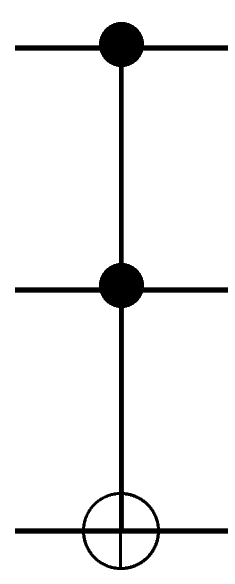
\includegraphics[width=0.1\textwidth]{img/ccnotcircuit.png}  & $\begin{pmatrix}
 \mathbb{1}_6 & 0 \\ 
 0 & X
 \end{pmatrix} = \begin{pmatrix}
 1 & 0 & 0 & 0 & 0 & 0 & 0 & 0 \\ 
 0 & 1 & 0 & 0 & 0 & 0 & 0 & 0 \\ 
 0 & 0 & 1 & 0 & 0 & 0 & 0 & 0 \\ 
 0 & 0 & 0 & 1 & 0 & 0 & 0 & 0 \\ 
 0 & 0 & 0 & 0 & 1 & 0 & 0 & 0 \\ 
 0 & 0 & 0 & 0 & 0 & 1 & 0 & 0 \\
 0 & 0 & 0 & 0 & 0 & 0 & 0 & 1 \\ 
 0 & 0 & 0 & 0 & 0 & 0 & 1 & 0 \\ 
 \end{pmatrix}$ & CCNOT($c_1$, $c_2$, target)\\\midrule
nCNOT & n-controlled NOT & 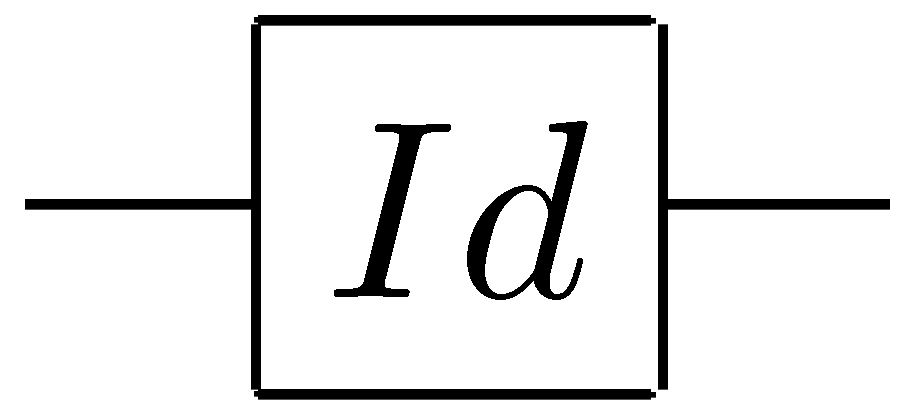
\includegraphics[width=0.1\textwidth]{img/identitycircuit.png}  & $\begin{pmatrix}
 \mathbb{1}_{2^n-2} & 0 \\ 
 0 & X
 \end{pmatrix}$ & nCNOT($c_1$,..,$c_n$, target) \\\midrule

\end{tabular}
\end{table}

\subsubsection{Toffoli Gate}
\label{subsubsubsec:toffoligate}

The most important three-qubit gate is a controlled controlled NOT (CCNOT) quantum gate which is often referred to as the Toffoli gate. It is defined by the following 8x8 matrix:
\begin{equation}
Toffoli = CCNOT = \begin{pmatrix}
 \mathbb{1}_6 & 0 \\ 
 0 & X
 \end{pmatrix} = \begin{pmatrix}
 1 & 0 & 0 & 0 & 0 & 0 & 0 & 0 \\ 
 0 & 1 & 0 & 0 & 0 & 0 & 0 & 0 \\ 
 0 & 0 & 1 & 0 & 0 & 0 & 0 & 0 \\ 
 0 & 0 & 0 & 1 & 0 & 0 & 0 & 0 \\ 
 0 & 0 & 0 & 0 & 1 & 0 & 0 & 0 \\ 
 0 & 0 & 0 & 0 & 0 & 1 & 0 & 0 \\
 0 & 0 & 0 & 0 & 0 & 0 & 0 & 1 \\ 
 0 & 0 & 0 & 0 & 0 & 0 & 1 & 0 \\ 
 \end{pmatrix}
\end{equation}

where $\mathbb{1}_6$ is the 6x6 identity matrix.

The Toffoli gate takes three inputs specified in parantheses, first the two control qubits and lastly the target qubit. If and only if both control qubits are in the \1 state the X gate is applied to the target qubit. Toffoli gates are usually decomposed into quantum circuits with CNOT and single-qubit gates in order to keep the set of quantum gates small \cite{shende2008cnot}.

\subsubsection{nCNOT Gate}
\label{subsubsubsec:ncnotgate}

The nCNOT gate is the generalization of the CNOT and the Toffoli gate. It takes $n$ control qubits and one target qubit as input and if and only if all control qubits are in the \1 state the X gate is applied to the target. The nCNOT matrix representation is given by:
 
\begin{equation}
nCNOT = \begin{pmatrix}
 \mathbb{1}_{2^n-2} & 0 \\ 
 0 & X
 \end{pmatrix}
\end{equation}

In practise, nCNOT gates are usually not implemented directly but decomposed into larger quantum circuits consisting only of CNOT and single-qubit gates \cite{nielsen2010quantum}. However, such decompositions will not be relevant for this work.


%%%%% SECTION: MACHINE LEARNING

\section{Classical Machine Learning}
\label{subsec:classicalmachinelearning}

\subsection{k-nearest Neighbour Algorithm}
\label{subsubsec:knearestneighbour}

Use text from proposal and slightly adapt.

\section{Methods (own chapter?)}
\label{subsec:methods}

\subsection{Programming environment}
\label{subsubsec:programming}

\subsection{IBMs QC}
\label{subsubsec:ibmqc}
\cleardoublepage
\chapter{Literature Review: Quantum-enhanced Machine Learning}\label{sec:qml}

Classical machine learning takes classical data as input and learns from it using classical algorithms executed on classical computers - this will be referred to as C/C (classical data with classical algorithm). One enters the field of quantum machine learning when either quantum data or quantum algorithms are combined with ideas from classical machine learning. Thus, quantum machine learning can be subdivided into three different subfields: 1) C/Q - classical data with quantum algorithm, 2) Q/C - quantum data with classical algorithm and 3) Q/Q - quantum data with quantum algorithm.

\emph{Quantum data} includes any data describing a quantum mechanical system such as e.g. the Hamiltonian of a system or the state vector of a certain quantum state. A \emph{quantum algorithm} is any algorithm that can only be executed on a quantum computer. 

C/Q is the topic of this thesis

Analogously, Q/C is the subfield where quantum data is being processed using a classical machine learning algorithm. Examples for Q/C:

used genetic algorithms to reduce digi-
tal and experimental errors in quantum gates

A tantamount task is then to
find a model (a.k.a. effective) Hamiltonian of the system
and to determine properties of the present noise sources.
By computing likelihood functions in an adaptation of
Bayesian inference, Wiebe et al. found that quan-
tum Hamiltonian learning can be performed using realis-
tic resources such as depolarizing noise.

Q/Q would include learning a model Hamiltonian of a system implemented in a lab using a quantum learning algorithm.

\subsection{Quantum State Preparation Algorithms}
\label{subsubsec:quantumstatepreparation}

\emph{Quantum state preparation} is the process of preparing a quantum state that accurately represents a vector containing classical (normalized) data. There are two fundamentally different ways of preparing a quantum state representing the classical example vector v:

\begin{equation}
\label{equ:v}
v = \begin{pmatrix}0.6 \\ 0.4 \end{pmatrix}
\end{equation}

\subsubsection{Encoding classical data into qubits}
\label{subsubsec:classicaldataqubits}
%speed-up not very clear since the \# of qubits increases linearly with the \# of classical bits
The most straightforward type of quantum state preparation does not make use of quantum superpositions but only uses the definite \0 or \1 states to store binary information in a multi qubit system as outlined in the example below.

Multiply vector v by ten such that the normalized entries can easily be represented in binary,
\begin{equation}
\begin{pmatrix}
 \textcolor{blue}{0.6} \\ 
 \textcolor{emerald}{0.4}
 \end{pmatrix}*10 = \begin{pmatrix}
 \textcolor{blue}{6} \\ 
 \textcolor{emerald}{4}
 \end{pmatrix}
\end{equation}
 Convert each entry to binary,
 \begin{equation}
 \begin{pmatrix}
 \textcolor{blue}{6} \\ 
 \textcolor{emerald}{4}
 \end{pmatrix} \rightarrow \begin{pmatrix}
 \textcolor{blue}{0110} \\ 
 \textcolor{emerald}{0100}
 \end{pmatrix}
 \end{equation}

 Rewrite the 2-D vector as a 1-D bit string,
 \begin{equation}
 \begin{pmatrix}
 \textcolor{blue}{0110} \\ 
 \textcolor{emerald}{0100}
 \end{pmatrix} \rightarrow n=\textcolor{blue}{0110}\textcolor{emerald}{0100}
\end{equation}
For $g$ bits initialize $g$ qubits in the \0 state \& apply the X gate to the respective qubits:
\begin{equation}
n=\textcolor{blue}{0110}\textcolor{emerald}{0100}  \rightarrow \ket{n} = (\textcolor{blue}{\mathbb{1} \otimes X \otimes X \otimes \mathbb{1}}\otimes\textcolor{emerald}{\mathbb{1} \otimes X \otimes \mathbb{1} \otimes \mathbb{1}})\ket{00000000} = \ket{\textcolor{blue}{0110}\textcolor{emerald}{0100}}
\end{equation}
%\textbf{Only slight speed up possible}

When encoding classical data into qubit states, a $k$-dimensional probability vector requires $4k$ classical bits which are encoded one-to-one into $4k$ qubits. Thus, the number of qubits increases linearly with the size of the classical data vector. Due to this one-to-one correspondence between classical bits and qubits there is no data compression improvement compared to classical data storage. Only slight (up to quadratic) speed-ups are possible through clever quantum algorithm design (CITATION).

Qubit-based quantum state preparation becomes slightly more complicated when aiming to achieve a quantum memory state $\ket{M}$ in an equal superposition of $l$ binary patterns $l^j$ of the form

\begin{equation}
\label{equ:memorysuperpos}
\ket{M} = \frac{1}{\sqrt{l}}\sum^l_{j=1} \ket{l^j}
\text{where } \ket{l^j} = \ket{l^j_1,l^j_2,...l^j_n} \text{and } l^j_k \in \left\{0,1\right\}
\end{equation}

Preparing this quantum state is a requirement for the later used qubit-encoded kNN quantum algorithm by \citeA{Schuld2014}. \citeA{Trugenberger2001} describe a quantum routine that can efficiently prepare such a state as will be explained in detail below.

First, \citeA{Trugenberger2001} defines the new unitary quantum gate $S^j$,

\begin{equation}
S^j = \begin{pmatrix}
\sqrt{\frac{j-1}{j}} & \frac{1}{\sqrt{j}} \\
-\frac{1}{\sqrt{j}} & \sqrt{\frac{j-1}{j}}
\end{pmatrix}
\end{equation}

and introduces its controlled version $CS^j$:

\begin{equation}
CS^j = \begin{pmatrix}
\mathbb{1} & 0 \\
0 & S^j
\end{pmatrix}
\end{equation}

The initial quantum state is given in Equ.~\ref{equ:truginitial} and consists of three registers; the first being the pattern register containing the first pattern $l^1$, the second register $u$ is a utility register initialized in state $\ket{01}$ and the third register $m$ represents the memory register initialized with $n$ zeros in which all patterns $l^j$ will be loaded one after the other.

\begin{equation}
\label{equ:truginitial}
\ket{\Psi^1_0} = \ket{l^1;u;m} = \ket{l^1_1,l^1_1,...,l^1_n;01;0_1,...,0_n} 
\end{equation}

The routine will use the second utility qubit $u_2$ to separate the intial state into two terms whereby $u_2 = \ket{0}$ flags the already stored patterns and $u_2 = \ket{1}$ indicates the processing term. In order to store a pattern $l^j$ in the memory register one has to perform the following operations:

\begin{bluebox}
Step 1: Using $u_2$ as one of the control qubits for the CCNOT gate, copy the pattern $l^j$ into the memory register of the processing term ($u_2=\ket{1}$):
\begin{equation}
\label{equ:trug1}
\ket{\Psi^j_1} = \prod_{r=1}^n CCNOT(l^j_r,u_2,m_r)\ket{\Psi^j_0} 
\end{equation}

Step 2: If the qubits in the pattern and memory register are identical (true only for the processing term) then overwrite all qubits in the memory register with ones:
\begin{equation}
\label{equ:trug2}
\ket{\Psi^j_2} = \prod_{r=1}^n X(m_r)CNOT(l^j_r,m_r)\ket{\Psi^j_1} 
\end{equation}

Step 3: Apply a nCNOT gate controlled by all $n$ qubits in the $m$ register and flip $u_2$ if and only if all $n$ qubits are ones (true only for the processing term):
\begin{equation}
\label{equ:trug3}
\ket{\Psi^j_3} = nCNOT(m_1,m_2,...,m_n,u_2)\ket{\Psi^j_2} 
\end{equation}

Step 4: Using the previously defined $CS^j$ operation, with control $u_1$ and target $u_2$ , the new pattern is transferred from the processing term into the term containing the already stored patterns ($u_2 = \ket{0}$):
\begin{equation}
\label{equ:trug4}
\ket{\Psi^j_4} = CS^{l+1-j}(u_1,u_2) \ket{\Psi^j_3} 
\end{equation}

Step 5 \& 6: In Step 2 \& 3 all qubits in the memory register were overwritten with ones and these steps can be undone by applying their inverse operations:
\begin{align}
\label{equ:trug56}
\ket{\Psi^j_5} &= nCNOT(m_1,m_2,...,m_n,u_2)\ket{\Psi^j_4} \\
\ket{\Psi^j_6} &= \prod_{r=n}^1 CNOT(l^j_r,m_r)X(m_r)\ket{\Psi^j_5} 
\end{align}

The resulting state is now given by the following equation:

\begin{equation}
\label{equ:trug6}
\ket{\Psi^j_6} = \frac{1}{\sqrt{l}} \sum^{j}_{w=1} \ket{l^j;00;l^w} + \sqrt{\frac{l-j}{l}} \ket{l^j;01;l^j}
\end{equation}

Step 7: Finally, by applying the inverse operation of Step 1 the memory register of the processing term is restored to zeros only:
\begin{equation}
\label{equ:trug7}
\ket{\Psi^j_7} = \prod_{r=n}^1 CCNOT(l^j_r,u_2,m_r) \ket{\Psi^j_6} 
\end{equation}
\end{bluebox}

At the end of Step 7 the next pattern can be loaded into the first register and by applying Steps 1-7 again the pattern gets added to the memory register. After repeating this procedure $l$ times the memory register $m$ will be in the desired state $\ket{M}$ defined by Equ.~\ref{equ:memorysuperpos}.

\subsubsection{Encoding classical data into amplitudes}
\label{subsubsec:classicaldataamplitudes}

A more sophisticated way of representing the classical vector $v$ (Equ.~\ref{equ:v}) as a quantum state makes use of the large number of available amplitudes in a multi qubit system. The general idea is demonstrated in Equ.~\ref{equ:amplitudedata} below.

\begin{equation}
\label{equ:amplitudedata}
\begin{pmatrix}
 \textcolor{blue}{0.6} \\ 
 \textcolor{emerald}{0.4}
 \end{pmatrix} \quad \rightarrow \quad \ket{n} = \sqrt{\textcolor{blue}{0.6}}\ket{0}+\sqrt{\textcolor{emerald}{0.4}}\ket{1}
\end{equation}

Using amplitude-based quantum state preparation, a $k$-dimensional probability vector is encoded into only $log_{2}(k)$ qubits since the number of amplitudes grows exponentially with the number of qubits. This type of quantum data storage makes exponential compression of classical data possible. Since a quantum gate acts on all amplitudes in the superposition at once there is the possibility of exponential speed-ups in quantum algorithms compared to their classical counterparts. Compared to the one-to-one correspondence in qubit-encoded state preparation, amplitude-encoding requires a much smaller number of qubits that grows logarithmically with the size of the classical data vector. However, initializing an arbitrary amplitude distribution is still an active field of research and requires the implementation of non-trivial quantum algorithms.

For the case when the classical data vectors represent discrete probability distributions which are efficiently integrable on a classical computer, \citeA{Grover2002} developed a quantum routine to initialize the corresponding amplitude distribution.
%The main idea in their algorithm is subdividing the respective probability distribution and encoding the probabilty
%VERY COMPLICATED AND MOST GENERAL
Additionally, \citeA{soklakov2006efficient} proposed a quantum algorithm for the more general case that includes initializing amplitude distributions for classical data vectors representing non-efficiently integrable probability distributions.

\subsection{Quantum k-nearest Neighbour Algorithm}
\label{subsubsec:quantumknearestneighbour}

The quantum distance-weighted kNN algorithm outlined in this section was proposed by \citeA{Schuld2014} and is based on classical data being encoded into qubits rather than amplitudes. The first step is to prepare an equal superposition $\ket{T}$ over $N$ training vectors $\vec{v}$ of length $n$ with binary entries $v_1,v_2,...v_n$ each assigned to a class $c$ as follows,

\begin{equation}
\label{equ:qubitknninitial}
\ket{T} = \frac{1}{\sqrt{N}}\sum_{p=1}^N \ket{v_1^p,v_2^p,...v_n^p;c^p}
\end{equation}

The unknown vector $\vec{x}$ of length $n$ and binary entries $x_1,x_2,...x_n$ needs to be classified and is added to the training superposition resulting in the initial state $\ket{\psi_0}$:

\begin{equation}
\ket{\psi_0} = \frac{1}{\sqrt{N}}\sum_{p=1}^N \ket{x_1,x_2,...x_n;v_1^p,v_2^p,...v_n^p;c^p}
\end{equation}

An ancilla qubit initially in state \0 is added to the state such that the superposition is now described by,

\begin{equation}
\ket{\psi_1} = \frac{1}{\sqrt{N}}\sum_{p=1}^N \ket{x_1,x_2,...x_n;v_1^p,v_2^p,...v_n^p;c^p} \otimes \ket{0}
\end{equation}

The state now consists of four registers: 1) input($x$) register, 2) training($v$) register, 3) class($c$) register and 4) ancilla($\ket{0}$) register. Next, the ancilla register is put into an equal superposition by applying an H gate to it,

\begin{align}
\ket{\psi_2} &= \frac{1}{\sqrt{N}}\sum_{p=1}^N \ket{x_1,x_2,...x_n;v_1^p,v_2^p,...v_n^p;c^p} \otimes H\ket{0}\notag\\
&= \frac{1}{\sqrt{N}}\sum_{p=1}^N \ket{x_1,x_2,...x_n;v_1^p,v_2^p,...v_n^p;c^p} \otimes \frac{(\ket{0}+\ket{1})}{\sqrt{2}}
\end{align}

The main step in any kNN algorithm is calculating some measure of distance between each training vector $\vec{v}$ and the input vector $\vec{x}$ which in this quantum algorithm is taken to be the Hamming distance defined in the red box below.

\begin{redbox}
\textbf{Hamming distance (CITATION?)}\\
\newline
Hamming distance (HD) is the number of differing characters when comparing two equally long binary patterns $p_0$ and $p_1$.\\
\newline
Example:\\
$p_0 = \quad\textcolor{red}{0}\quad\textcolor{green}{0\quad1}$\\
$p_1 = \quad\textcolor{red}{1}\quad\textcolor{green}{0\quad1}$\\
$--------$\\
HD $= 1+0+0 = 1$
\end{redbox}

Given quantum state $\ket{\psi_2}$ the HD between the input and each training register can be calculated by applying CNOT($x_s,v_s^p$) gates to all qubits in the first and second register using the input vector qubits $x_s$ as controls and the training vector qubits $v_s^p$ as targets. This will change the qubits in the second register according to the rules specified in Equ.~\ref{equ:distancerules}. 

\begin{equation}
\label{equ:distancerules}
d^p_s =
    \begin{cases}
      0, & \text{if}\ \ket{v_s^p} = \ket{x_s} \\
      1, & \text{otherwise}
    \end{cases}
\end{equation}

The sum of the qubits in the second register now represents the total HD between each training register and the input. Applying an X gate to each qubit in the second register reverses the HD such that small HDs become large and vice versa. This is crucial since training vectors close to the input should get larger weights than more distant vectors. The quantum state is now given by,

\begin{align}
\ket{\psi_3} &= \prod_{s=1}^n X(v^p_s)CNOT(x_s,v^p_s)\ket{\psi_2}\notag\\
&= \frac{1}{\sqrt{N}}\sum_{p=1}^N \ket{x_1,x_2,...x_n;d_1^p,d_2^p,...d_n^p;c^p} \otimes \frac{(\ket{0}+\ket{1})}{\sqrt{2}}
\end{align}

By applying the unitary operator $U$ defined by,

\begin{equation}
\label{equ:sumoperator}
U = e^{-i\frac{\pi}{2n}K}
\end{equation}

where

\begin{equation}
\label{equ:sumoperator}
K = \mathbb{1} \otimes \sum_s (\frac{\sigma_z+1}{2})_{d_s} \otimes \mathbb{1} \otimes (\sigma_z)_c
\end{equation}

the sum over the second register is computed. As a result, the total reverse HD, denoted $d_H(\vec{x},\vec{v}^p)$, between the $p$th training vector $\vec{v}^p$ and the input vector $\vec{x}$ is written into the complex phase of the p$th$ term in the superposition. The ancilla register is now separating the superposition into two terms due to a sign difference in the amplitudes (negative sign when ancilla is \1). The result is given by, 

\begin{align}
\ket{\psi_4} &= U\ket{\psi_3}\notag\\
&= \frac{1}{\sqrt{2N}}\sum_p^N e^{i\frac{\pi}{2n}d_H(\vec{x},\vec{v}^p)} \ket{x_1,x_2,...x_n;d_1^p,d_2^p,...d_n^p;c^p;0} \notag\\
&\quad\quad\quad\quad\quad\quad + e^{-i\frac{\pi}{2n}d_H(\vec{x},\vec{v}^p)} \ket{x_1,x_2,...x_n;d_1^p,d_2^p,...d_n^p;c^p;1}
\end{align}

Applying an H gate to the ancilla register transfers the $d_H(\vec{x},\vec{v}^p)$ from the phases into the amplitudes such that the new quantum state is described by,

\begin{align}
\label{equ:beforecm}
\ket{\psi_5} &= (\mathbb{1} \otimes \mathbb{1} \otimes \mathbb{1} \otimes H)\ket{\psi_4}\notag\\
&= \frac{1}{\sqrt{N}}\sum_p^N cos\big[\frac{\pi}{2n}d_H(\vec{x},\vec{v}^p)\big] \ket{x_1,x_2,...x_n;d_1^p,d_2^p,...d_n^p;c^p;0} \notag\\
&\quad\quad\quad\quad\quad\quad + sin\big[\frac{\pi}{2n}d_H(\vec{x},\vec{v}^p)\big] \ket{x_1,x_2,...x_n;d_1^p,d_2^p,...d_n^p;c^p;1}
\end{align}

At this point the ancilla qubit is measured along the standard basis and all previous steps have to be repeated until the ancilla is measured in the \0 state. Since it is conditioned on a particular outcome, this type of measurement is called \emph{conditional measurement} (CM). The probability of a successful CM is given by the square of the absolute value of the amplitude and is dependent on the average reverse HD between all training vectors and the input vector:

\begin{equation}
Prob(\ket{a} = \ket{0}) = \sum_p^N cos^2\big[\frac{\pi}{2n}d_H(\vec{x},\vec{v}^p)\big]
\end{equation}

Finally, to classify the input vector $\vec{x}$ the class register is measured along the standard basis. The probability of measuring a specific class c is then given by the following expression:

\begin{equation}
\label{equ:classprobs}
Prob(c) = \frac{1}{NProb(\ket{a} = \ket{0})} \sum_{l \in c} cos^2\big[\frac{\pi}{2n}d_H(\vec{x},\vec{v}^l)\big]
\end{equation}

%When rewriting Equ.~\ref{equ:beforecm} into the following form,

%\begin{align}
%\label{equ:beforecm2}
%\ket{\psi_5} &= \frac{1}{\sqrt{N}}\sum_{c=1}^d \ket{c} \otimes \sum_{l \in c} cos\big[\frac{\pi}{2n}d_H(\vec{x},\vec{v}^l)\big] \ket{x_1^l,x_2^l,...x_n^l;d_1^l,d_2^l,...d_n^l;0} \notag\\
%&\quad\quad\quad\quad\quad\quad\quad\quad\quad\quad + sin\big[\frac{\pi}{2n}d_H(\vec{x},\vec{v}^l)\big] \ket{x_1^l,x_2^l,...x_n^l;d_1^l,d_2^l,...d_n^l;1}
%\end{align}

%where $l$ runs over all vectors $\vec{v}$ of a particular class c.

From Equ.~\ref{equ:classprobs} it is evident that the probability of measuring a certain class $c$ is dependent on the average total reverse HD between all training vectors belonging to class $c$ and the input vector $\vec{x}$. Since the total reverse HD represent distance-dependent weights it gets clear why this is the quantum equivalent to a classical distance-weighted kNN algorithm.

In order to obtain a full picture of the probability distribution over the different classes a sufficient number of copies of $\ket{\psi_5}$ needs to be prepared and after successful CM on the ancilla qubit the class qubit needs to be measured.

\begin{redbox}
\textbf{Algorithmic complexity}\\
\newline
According to \citeA{Schuld2014}, the preparation of the superposition has a complexity of $\mathcal{O}(Pn)$ where $P$ is the number of training vectors and $n$ is the length of the feature vectors. The algorithm has to be repeated $T$ times in order to get a statistically precise picture of the results. Hence, the total quantum kNN algorithm has an algorithmic complexity of $\mathcal{O}(TPn)$. 
\end{redbox}


\cleardoublepage
%\chapter{Results and Discussion}\label{sec:resultsanddiscussion}


\subsubsection{Diffusion matrix from quantum random walks}
\label{subsubsubsec:diffusion}

For the simplest case, consider the entries in the classical probability vector v to be normal distributed, e.g.

CHECK THE ORDER!
\begin{equation}
v = \colvec{0.064180\\0.146860\\0.146770\\0.341590\\0.026840\\0.063590\\0.061700\\0.148470}
\end{equation}

The goal is to encode this classical data into a quantum memory state $\ket{M}$ of the form,

\begin{align}
\ket{M} = \quad &0.064180 \ket{000} +
0.146860 \ket{100} +
0.146770 \ket{010} +
0.341590 \ket{001}\notag\\
&+ 0.026840 \ket{110}
+ 0.063590 \ket{011} +
0.061700 \ket{101} +
0.148470 \ket{111}
\end{align}

%Before outlining how to prepare state $\ket{M}$ the notion of Hamming distance needs to be introduced.

Furthermore, a useful tool of visualizing the HDs between binary patterns made from three qubits is a 3-D cube as shown in Fig.~\ref{img:cubenoprobs}. On the cube, adjacent qubit patterns have a HD of 1 and the HD increases by 1 for every additional corner. For example, the qubit state $\ket{000}$ is adjacent to $\ket{100}$ since they only differ in one qubit ($HD=1$). Moving one more corner yields the state $\ket{101}$ or $\ket{110}$ which both have a HD of 2 compared to $\ket{000}$.

\begin{figure}[!ht]
       \centering
       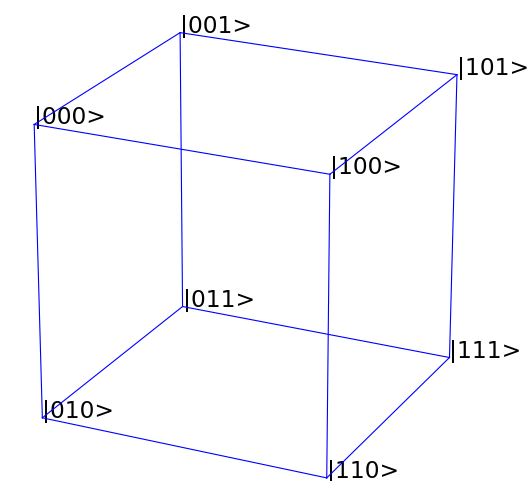
\includegraphics[width=0.5\textwidth]{img/cubewithoutprobs.png}
       \caption{\label{img:cubenoprobs} Visualizing Hamming distances on a 3-D cube}
\end{figure}

This way of visualizing HDs can be extended to the 16 binary patterns made by four qubits that can be visualized on a 4-D cube, also called tesseract, as illustrated in Fig.~\ref{img:hypercubenoprobs}.

\begin{figure}[!ht]
       \centering
       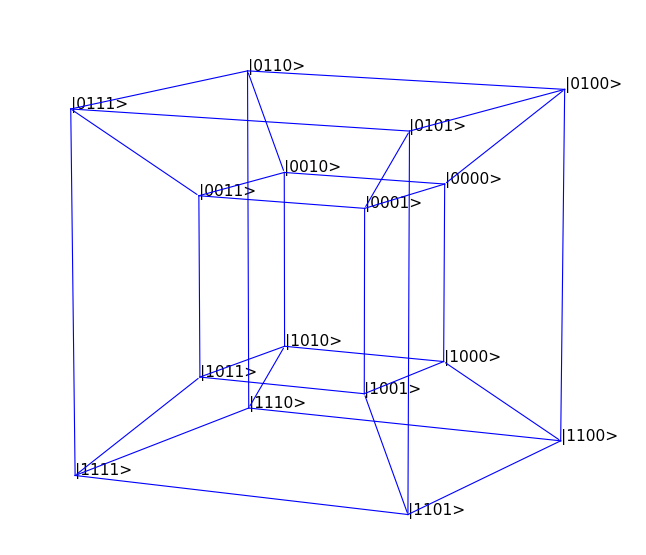
\includegraphics[width=0.5\textwidth]{img/hypercubewithoutprobs.png}
       \caption{\label{img:hypercubenoprobs} Visualizing Hamming distances on a 4-D cube (tesseract)}
\end{figure}

The idea of a coin operator $C$ can be borrowed from the theory of quantum random walks to initialize a gaussian distribution centered around a chosen binary qubit pattern. For this purpose, the coin operator is defined as,

\begin{equation}
C = \begin{pmatrix}
\sqrt{\delta} & 1-\sqrt{\delta} \\
1-\sqrt{\delta} & -\sqrt{\delta}
\end{pmatrix}
\end{equation}

where $0 \leq \delta \leq 1$.


\subsubsection{Amplitude-based quantum kNN algorithm}
\label{subsubsubsec:quantumknearestneighbouramplitudes}

\begin{equation}
\frac{1}{\sqrt{2M}}\sum_{m=1}^{M} (\textcolor{emerald}{\ket{0}}\ket{\textcolor{red}{\Psi_{\tilde{x}} (\star)}}+\textcolor{emerald}{\ket{1}}\ket{\textcolor{darkyellow}{\Psi}_{\textcolor{purple}{x^{m}}}})\ket{y^{m}(\textcolor{darkyellow}{A} \ or \ \textcolor{purple}{B})}\ket{m}
\end{equation}
where
\begin{equation}
\ket{\textcolor{red}{\Psi_{\tilde{x}} (\star)}} = \sum_{i=1}^{N} \textcolor{red}{\tilde{x}_i}\ket{i} \quad \quad
\ket{\textcolor{darkyellow}{\Psi}_{\textcolor{purple}{x^{m}}}}	 = \sum_{i=1}^{N} \textcolor{darkyellow}{x}\textcolor{purple}{_i^m} \ket{i} 
\end{equation}

\begin{equation}
e.g. \quad \begin{pmatrix}
 \textcolor{blue}{0.6} \\ 
 \textcolor{emerald}{0.4}
 \end{pmatrix} \quad \rightarrow \quad \ket{n} =  \sqrt{\textcolor{blue}{0.6}}\ket{0}+\sqrt{\textcolor{emerald}{0.4}}\ket{1}
\end{equation}

Applying the \textbf{Hadamard gate} interferes the input and the training vectors:

\begin{equation}
\frac{1}{2\sqrt{M}}\sum_{m=1}^{M} (\textcolor{emerald}{\ket{0}}[\ket{\textcolor{red}{\Psi_{\tilde{x}}}}+\ket{\textcolor{darkyellow}{\Psi}_{\textcolor{purple}{x^{m}}}}]+\textcolor{emerald}{\ket{1}}[\ket{\textcolor{red}{\Psi_{\tilde{x}}}}-\ket{\textcolor{darkyellow}{\Psi}_{\textcolor{purple}{x^{m}}}}])\ket{y^{m}(\textcolor{darkyellow}{A} \ or \ \textcolor{purple}{B})}\ket{m}
\end{equation}

$\rightarrow$ Perform \textbf{conditional measurement} on ancilla qubit.\\
Successful if $\ket{0}$ state is measured.

After successful conditional measurement, the state is proportional to
\begin{equation}
\frac{1}{2\sqrt{M}}\sum_{m=1}^{M} \sum_{i=1}^{N} (\textcolor{red}{\tilde{x}_i}+\textcolor{darkyellow}{x}\textcolor{purple}{_i^m})\ket{0}\ket{i}\ket{y^{m}(\textcolor{darkyellow}{A} \ or \ \textcolor{purple}{B})}\ket{m}
\end{equation}

Probability to measure class B:
\begin{equation}
p(\ket{y^m} = \ket{1(\textcolor{purple}{B})})= \sum_{m \mid y^m=1(\textcolor{purple}{B})} 1 - \frac{1}{4M} \mid \textcolor{red}{\tilde{x}} - \textcolor{purple}{x^m} \mid ^2
\end{equation}

Hereby, the advantages of the quantum version are the parallel computation of the distances between each training vector and the input vector as well as contracting distance computation and distance weighting into one computational step.

The quantum advantage of the algorithm is the simultaneous computation of the HD between the input vector and each training vector which is impossible to do classically. For example, if the training set contains 1,000,000 vectors with 10 entries each, the quantum algorithm performs all 1,000,000 distance computations with the application of only 10 X and 10 CNOT gates. In contrast, the classical algorithm would need to perform  1,000,000 individual computations in order to be able to apply distance-dependent weights to each training vector. 


\subsubsection{Controlled U Gate}
\label{subsubsubsec:controlledugate}

Often there is a need for applying certain quantum gates in a controlled manner. Thus a controlled U (CU) gate is required whereby U can be any unitary single-qubit gate. The CU gate is defined as:

\begin{equation}
CU = \begin{pmatrix}
 \mathbb{1} & 0 \\ 
 0 & U
 \end{pmatrix}
\end{equation}

It is important to note that the CNOT gate is essentially a CU gate in the case of U = X. 

Most of the time the CU gate cannot be implemented directly and has to be realized through larger quantum circuits consisting of CNOT and single-qubit gates. \citeA{nielsen2010quantum} describe such a decomposition as shown in Fig.~\ref{img:cudecomposition}.

\begin{figure}[ht]
   \centering
   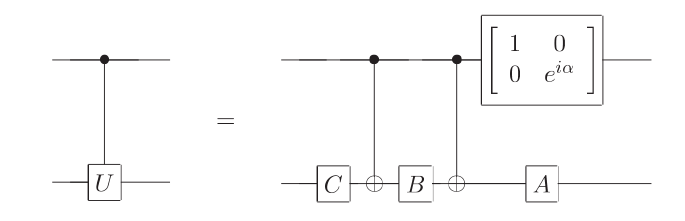
\includegraphics[width=0.7\textwidth]{img/controlledudecomp.png}
   \caption{Circuit decomposition for a controlled-U operation for single-qubit gate U.\textsuperscript{3}}
   \label{img:cudecomposition}
\end{figure}

\footnotetext[3]{Reprinted from Michael A. Nielsen and Isaac L. Chuang. Quantum Computation and Quantum Information. Cambridge University Press, 2000. Copyright 2010 by Nielsen \& Chuang.}

The idea is that when the control qubit is \0 the gate combination ABC is applied to the target qubit and has to equal the identity gate:

\begin{equation}
ABC = \mathbb{1}
\end{equation}

If and only if the control qubit is \1 then the gate sequence $e^{i\alpha}AXBXC$ is applied to the target. Since the goal is to apply the unitary U to the target qubit the following equation must be satified,

\begin{equation}
e^{i\alpha}AXBXC = U
\end{equation}

In order to find the matrices A,B,C and the additional parameter $\alpha$ the following equation has to be solved:

\begin{equation}
U = \begin{pmatrix}
 e^{i(\alpha-\frac{\beta}{2}-\frac{\delta}{2})}\cos{\frac{\gamma}{2}} & -e^{i(\alpha-\frac{\beta}{2}+\frac{\delta}{2})}\sin{\frac{\gamma}{2}} \\ 
e^{i(\alpha+\frac{\beta}{2}-\frac{\delta}{2})}\sin{\frac{\gamma}{2}} & e^{i(\alpha+\frac{\beta}{2}+\frac{\delta}{2})}\cos{\frac{\gamma}{2}}
 \end{pmatrix}
\end{equation}
%\cleardoublepage
%\chapter{Outlook}\label{sec:outlook}
%\cleardoublepage
%\chapter{Conclusion}\label{sec:conclusion}

Quantum-enhanced machine learning aims to harness the properties of quantum mechanical systems to enhance the performance of classical machine learning algorithms beyond the reach of classical computers. This becomes increasingly important since big data pushes computational resources and classical algorithms to their limits. This research established proof-of-principle simulations of two variants of a distance-weighted quantum $k$-nearest neighbour (kNN) algorithm using three small-scale supervised machine learning tasks.
%However, current quantum computing efforts have not yet led to the construction of a large-scale universal quantum computer and, thus, most of the current quantum-enhanced machine learning research is purely theoretical. Yet, small-scale quantum computers have been realised already and up to 30 qubits can still be simulated on a conventional laptop. Thus, this research is part of the attempt to shift quantum-enhanced machine learning into a more applied field by establishing proof-of-principle simulations of two variants of a distance-weighted quantum $k$-nearest neighbour (kNN) algorithm using three small-scale supervised machine learning tasks.
%On the other hand, IBM has enabled public access to their five-qubit quantum computer and small quantum computers with up to 30 qubits can still be simulated on conventional laptops. 

Firstly, the qubit-based kNN algorithm by \citeA{Schuld2014} was combined with a quantum state preparation routine by \citeA{Trugenberger2001} to classify various 9-bit RGB colours into the classes \emph{red} and \emph{blue}. Microsoft's software architecture Liqui$\ket{}$ was used to simulate the algorithm on two levels of difficulty. In the easy evaluation stage, the quantum kNN achieved a classification accuracy of 75\% which was subsequently raised to 100\% in the more challenging evaluation stage with a larger training dataset. These results show that the qubit-based kNN routine is a very effective classification algorithm concerning 9-bit RGB colours.

Aiming for an implementation with the IBM Quantum Experience, an amplitude-based kNN algorithm (aKNN) was developed by \citeA{SchuldFingerhuth}.  A simple binary Bloch vector classification tasks was considered to keep the requirements on the quantum hardware as small as possible. The necessary quantum compiling steps mapping the quantum state preparation routine and the aKNN algorithm to the IBM quantum hardware were outlined. For that particular classification task, it was shown that it could not be implemented within IBM's 40 quantum gate slots. Even though an implementation might be feasible using different datasets, the research demonstrated that there are cases which require relatively large gate sequences for implementation. As an alternative, the Bloch vector classification problem using the aKNN algorithm was simulated in Liqui$\ket{}$. The simulated algorithm led to the correct classification of two Bloch vectors. Lastly, the aKNN algorithm was simulated for the classification of discrete Gaussian distributions constituting a higher-dimensional classification problem using a slightly more advanced quantum state preparation routine. The simulated algorithm classified 83.3\% of various discrete Gaussian distributions correctly.

Overall, the Liqui$\ket{}$ quantum simulations clearly demonstrated the effectiveness of both quantum kNN algorithms. When combined with more general quantum state preparation routines, these algorithms bear the potential to speed up the processing of big data. Thus, a breakthrough in the development of a universal quantum computer would not solely constitute a major milestone in physics but most probably also revolutionise the field of machine learning.

%\cleardoublepage
%\chapter{Personal Reflection}\label{sec:personalreflection}

Personally, this bachelor thesis research has been instructive and beneficial in many different ways. Most importantly, I have had the opportunity to dedicate my entire time to learn about the subject of quantum information and, specifically, quantum machine learning in detail. Since these subjects are not taught within the curriculum of the Maastricht Science Programme (MSP) it was especially amazing to challenge myself to these notoriously difficult subjects within the intersection of quantum physics and computer science. In doing so, I have learned more about the methods of theoretical physics and gained additional experience in scientific programming with Octave, Python and F\#. Without prior knowledge of F\#, I was able to learn how to simulate quantum computations and quantum machine learning algorithms using the quantum simulation toolsuite Liqui$\ket{}$. Furthermore, I was able to use the first cloud-based quantum computer, the so-called IBM Quantum Experience, publicly released in May 2016 by IBM.

Alongside my research, I had the possibility to attend many great lectures, seminars and three conferences which were all generously funded by the Centre for Quantum Technology. This enabled me to get to know many renowned scientists working in the fields of quantum information, quantum machine learning, open quantum systems, quantum optics and quantum cryptography. Furthermore, I was provided with the opportunity to present my research at the 4\textsuperscript{th} South African conference for quantum information processing, communication and control in Cape Town in late November 2016. This constituted a big step with respect to my academic career and a great way of putting my acquired presentation skills to practice.

However, in retrospective I feel that I could have been more productive in office by structuring my work days more diligently. For example, the first one and a half months were mostly spent on reading research paper and text books to acquire the theoretical foundation for my research and little time was used to practice F\# within the Liqui$\ket{}$ framework. A possible solution for the future would be to divide each day into two parts: e.g. spending the morning with reading papers and books and the afternoon on practical work and programming. Besides this, I feel like I should have communicated my progress more with my internal supervisor Dr. Birembaut at the MSP.

In conclusion, the bachelor thesis research has showed me the importance of interdisciplinarity since the field of quantum information requires the understanding of concepts in computer science as well as quantum mechanics. Fortunately, MSP's liberal education does not only focus on textbook exercises and lectures but mostly teaches us how to systematically approach unknown topics and tackle problems therein. It was great to see that this enabled me to venture into a previously unfamiliar field and learn the necessary skills to conduct meaningful research. The newly acquired skills will certainly be useful for my planned masters in the field of quantum information.

%During the thesis work, I realized that encountering problem after problem is at the core of research but that one can resolve most of them when just showing enough dedication.

%The Centre for Quantum Technology at the University of KwaZulu-Natal in South Africa has been a wonderful host for my Bachelor thesis research. My supervisor Prof. Francesco Petruccione has become a mentor and friend and provided me with great opportunities for personal and academic growth. Furthermore, my collaborator Maria Schuld has shared vasts amount of knowledge, tricks and ideas with me and has always been a great help during my research work. Alongside my research, I had the possibility to attend many great lectures, seminars and three conferences which were all generously funded by the Centre for Quantum Technology. This enabled me to get to know many renowned scientists working in the fields of quantum information, quantum machine learning, open quantum systems, quantum optics and quantum cryptography. Attending the Quantum Machine Learning Workshop at the Dolphin Coast in July 2016 provided me with a broad overview of the field of quantum machine learning and was the first time that I ever attended a scientific conference. In November 2016, I was provided with the opportunity to present my research at the 4\textsuperscript{th} South African conference for Quantum Information Processing, Communication and Control in Cape Town. This opened the possibility for a collaboration with an experimental research group in Israel working on quantum computation with trapped ions. In January 2017, I am invited to the NiTheP Chris Engelbrecht Quantum Machine Learning Summer School where I will give three workshop sessions on quantum machine learning using the Liqui$\ket{}$ framework and the IBM Quantum Experience.
%\cleardoublepage
%\chapter{Working with \LaTeX\ }\label{sec:working}
This chapter explains how to typeset some of the most common elements contained in a technical report using \LaTeX.

\section{Headings}
Your report can be structured using several different types of headings. Use the commands \texttt{\textbackslash chapter\{.\}}, \texttt{\textbackslash section\{.\}}, \texttt{\textbackslash subsection\{.\}}, and \texttt{\textbackslash subsubsection\{.\}}. Use the asterisk symbol \texttt{*} to suppress numbering of a certain heading if necessary, for example, \texttt{\textbackslash section*\{.\}}.

\section{References and Footnotes}\label{sec:references}
References to literature are included using the command \texttt{\textbackslash
cite\{.\}}. For example \cite{optreg,motsys}. Your references must be entered in the file \texttt{bibliography.bib}. Making changes or adding new references in the bibliography file can be done manually or by using specialized software such as \textit{JabRef} which is free of charge.
 
Cross-referencing within the text is easily done using \texttt{\textbackslash label\{.\}} and \texttt{\textbackslash ref\{.\}}. For example, this paragraph is part of chapter~\ref{sec:working}; more specifically section~\ref{sec:references} on page~\pageref{sec:references}. You will need to compile your document twice in order for the cross-referencing to be updated.

Footnotes\footnote{The use of footnotes is generally not recommended.} are added using the command \texttt{\textbackslash footnote\{.\}}, but try to avoid the used of footnotes altogether.

\section{Lists}\label{sec:lists}
Three types of list-environments are commonly used: \texttt{itemize}, \texttt{enumerate}, and \texttt{description}. The following example uses \texttt{itemize} to create a list without numbering
\begin{itemize}
  \item point one; and
  \item point two
\end{itemize}
created using
\begin{verbatim}
\begin{itemize}
  \item point one; and
  \item point two
\end{itemize}
\end{verbatim}

The following example uses \texttt{enumerate} to create a list with numbering
\begin{enumerate}
  \item point one; and
  \item point two
\end{enumerate}
created using
\begin{verbatim}
\begin{enumerate}
  \item point one; and
  \item point two
\end{enumerate}
\end{verbatim}

The following example uses \texttt{description} to create a list with custom text as bullet-points
\begin{description}
  \item[P1] point one; and
  \item[P2] point two
\end{description}
created using
\begin{verbatim}
\begin{description}
  \item[P1] point one; and
  \item[P2] point two
\end{description}
\end{verbatim}


\section{Tables}\label{sec:tables}
Table~\ref{tab:table} shows an example of a simple table-layout. Try to avoid vertical lines on tables. The Internet contains countless resources on how to create special elements and structures in tables such as cells spanning multiple rows, rotated text, sideways tables, justification of cell elements, etc.
\begin{table}[ht]
\begin{center}
\caption{Driving cycle data of ECE-15, EUDC, and NEDC.}\vspace{1ex}
\label{tab:table}
\begin{tabular}{llccc}\hline
Description & Unit & ECE & EUDC & NEDC \\ \hline
Duration & s & 780 & 400 & 1180 \\
Distance & km & 4.052 & 6.955 & 11.007 \\
Average velocity & km/h & 18.7 &  62.6 & 33.6 \\
Idle speed & \% & 36 & 10 & 27 \\ \hline
\end{tabular}
\end{center}
\end{table}

This table was created using
\begin{verbatim}
\begin{table}[ht]
\begin{center}
\caption{Driving cycle data of ECE-15, EUDC, and NEDC.}\vspace{1ex}
\label{tab:table}
\begin{tabular}{llccc}\hline
Description & Unit & ECE & EUDC & NEDC \\ \hline
Duration & s & 780 & 400 & 1180 \\
Distance & km & 4.052 & 6.955 & 11.007 \\
Average velocity & km/h & 18.7 &  62.6 & 33.6 \\
Idle speed & \% & 36 & 10 & 27 \\ \hline
\end{tabular}
\end{center}
\end{table}
\end{verbatim}
Table~\ref{tab:table_advanced} shows a more advanced version of Tab.~\ref{tab:table} using the \texttt{booktabs} package. Inspect the source code of this document to see how this was done.
\begin{table}[ht]
\begin{center}
\small
\caption{Driving cycle data of ECE-15, EUDC, and NEDC.}\vspace{1ex}
\label{tab:table_advanced}
\begin{tabular}{@{}lcccc@{}}\toprule[1.5pt]
& & \multicolumn{3}{c}{\bf Driving cycle}\\
\cmidrule{3-5}
Description & Unit & {ECE} & {EUDC} & {NEDC} \\ \midrule
Duration & \unit[]{s} & 780 & 400 & 1180 \\
Distance & \unit[]{km} & 4.052 & 6.955 & 11.007 \\
Average velocity & \unitfrac[]{km}{h} & 18.7 &  62.6 & 33.6 \\
Idle speed & \unit[]{\%} & 36 & 10 & 27 \\ \bottomrule[1.5pt]
\end{tabular}
\end{center}
\end{table}



\section{Working with Units}
The package \texttt{\textbackslash usepackage\{units\}} enables two useful commands, namely \texttt{\textbackslash unit[.]\{.\}} and \\ \texttt{\textbackslash unitfrac[.]\{.\}\{.\}}. Use these commands to display units in a concise way, for example
\begin{align}
\delta t &= \unit[1]{s}\\
v &= \unitfrac[5]{m}{s}.
\end{align}
This example was done using
\begin{verbatim}
\begin{align}
\delta t &= \unit[1]{s}\\
v &= \unitfrac[5]{m}{s}.
\end{align}
\end{verbatim}

\section{Including Graphics}\label{sec:epsgraph}
It is recommended that you only use encapsulated post-script graphics \texttt{.eps} in your report. If you mix \texttt{.eps} with other formats such as \texttt{.png}, \texttt{.jpeg} or \texttt{.gif}, you will most likely not be able to compile your report without errors. Note that figures created in \textsc{Matlab} are easily saved in \texttt{.eps} format.

The inclusion of a figure can be done in the following way:
\begin{verbatim}
\begin{figure}[ht]
   \centering
   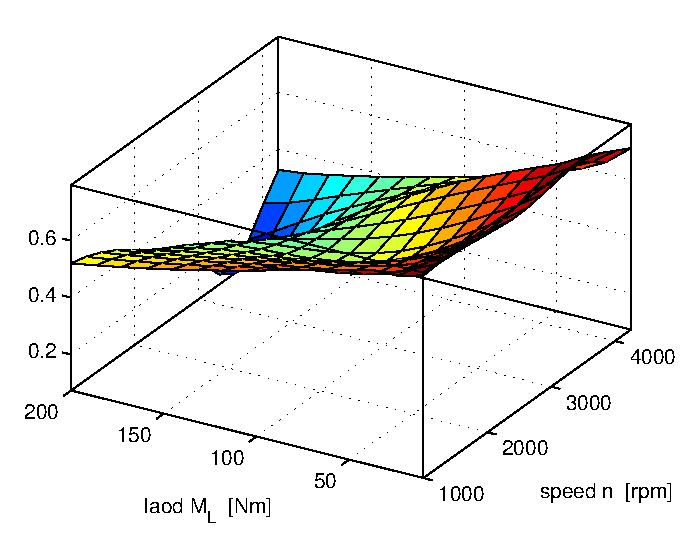
\includegraphics[width=0.75\textwidth]{img/k_surf.eps}
   \caption{Example of a figure.}
   \label{img:k_surf}
\end{figure}
\end{verbatim}

\begin{figure}[ht]
   \centering
   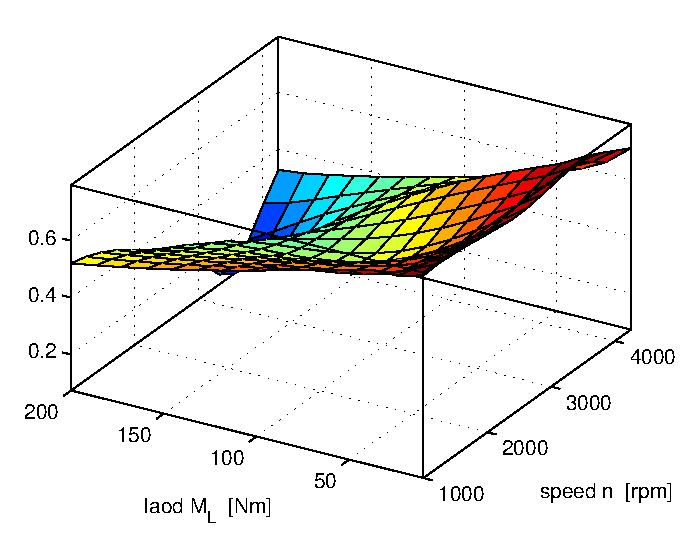
\includegraphics[width=0.75\textwidth]{img/k_surf.eps}
   \caption{Example of a figure.}
   \label{img:k_surf}
\end{figure}

Two figures are displayed next to each other using
\begin{verbatim}
\begin{figure}[ht]
  \begin{minipage}[t]{0.48\textwidth}
    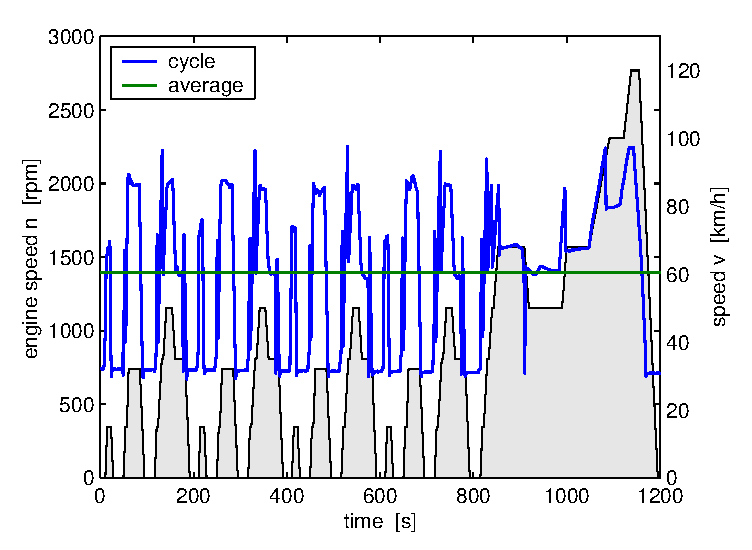
\includegraphics[width = \textwidth]{img/cycle_we.eps}
  \end{minipage}
  \hfill
  \begin{minipage}[t]{0.48\textwidth}
    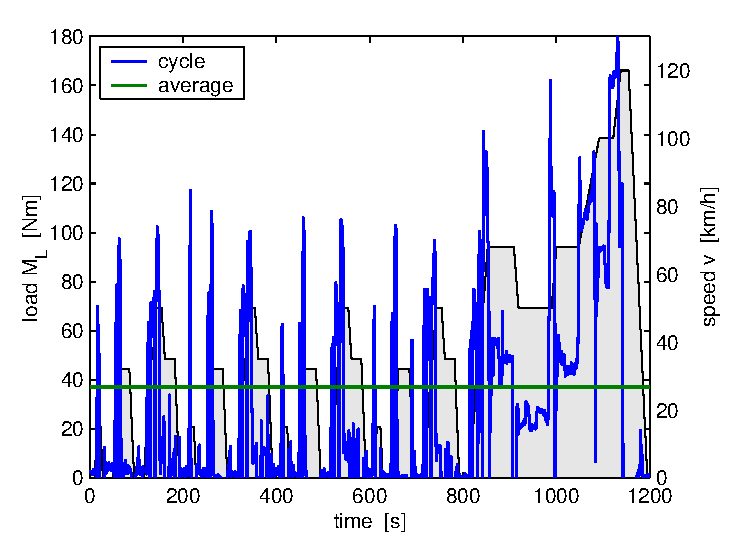
\includegraphics[width = \textwidth]{img/cycle_ml.eps}
  \end{minipage}
  \caption{Two figures next to each other.}
  \label{img:cycle}
\end{figure}
\end{verbatim}

\begin{figure}[ht]
  \begin{minipage}[t]{0.48\textwidth}
    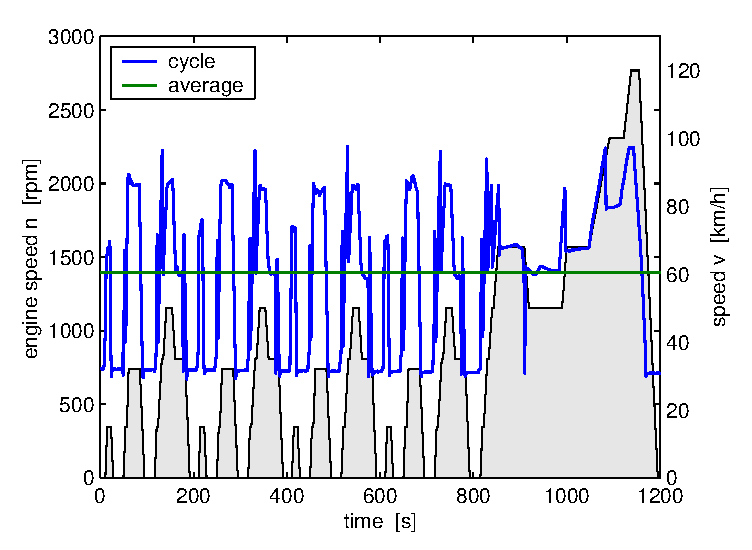
\includegraphics[width = \textwidth]{img/cycle_we.eps}
  \end{minipage}
  \hfill
  \begin{minipage}[t]{0.48\textwidth}
    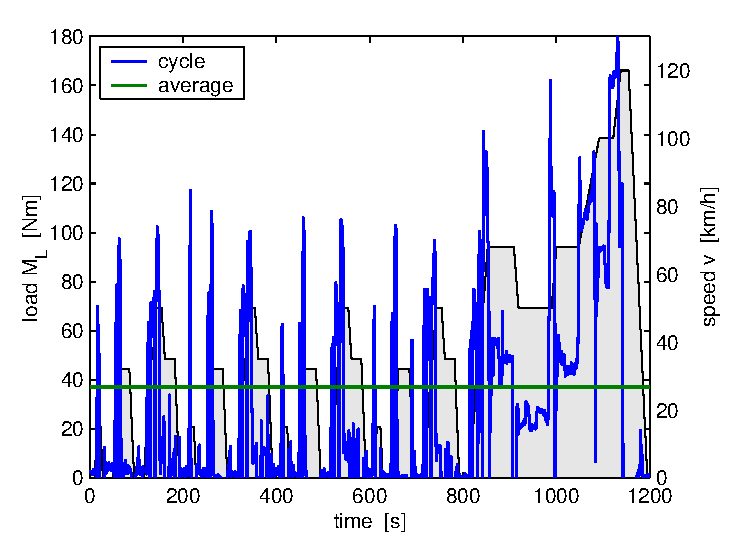
\includegraphics[width = \textwidth]{img/cycle_ml.eps}
  \end{minipage}
  \caption{Two figures next to each other.}
  \label{img:cycle}
\end{figure}

The positioning parameter \texttt{h} (here) forces your figure to be placed in the current position relative to your text. You may add \texttt{t} (top), \texttt{b} (bottom), and/or \texttt{p} (page) to allow for more flexible positioning within your document. For instance, \texttt{[tb]} forces your figure to be placed either on the top or bottom of a page.


\section{Equations}\label{sec:math}
The most common way to include equations is using the \texttt{equation} environment.
\begin{equation}\label{eq:p_me0f}
 p_\mathrm{me0f}(T_e,\omega_e) \ = \ k_1(T_e) \cdot (k_2+k_3 S^2
 \omega_e^2) \cdot \Pi_\mathrm{max} \cdot \sqrt{\frac{k_4}{B}} \, .
\end{equation}
It is recommended to use \texttt{\textbackslash mathrm\{.\}} for subscripts comprising more than two letters since it reduces the width of the subscript significantly and improves readability. The corresponding code is
\begin{verbatim}
\begin{equation}\label{eq:p_me0f}
 p_\mathrm{me0f}(T_e,\omega_e) \ = \ k_1(T_e) \cdot (k_2+k_3 S^2
 \omega_e^2) \cdot \Pi_\mathrm{max} \cdot \sqrt{\frac{k_4}{B}} \, .
\end{equation}
\end{verbatim}
Equations, such as Eq.~\eqref{eq:p_me0f}, may be referenced using \texttt{\textbackslash eqref\{.\}}. In-line mathematical content is created using \texttt{\$.\$}, for example $a^2+b^2=c^2$. It is practically possible to typeset any equation in \LaTeX. Equation~\eqref{eq:advanced} shows an example of a more advance structure.
\begin{equation}\label{eq:advanced}
x^k_n(i) = \left\{\begin{array}{ll}y(i) & \text{if}\quad x^k_{n-1}(i)\leq \mathbf{x}\\
z(i) & \text{otherwise}\end{array}\right., \text{for}\quad i=\{1,\ldots,N\}.
\end{equation}



\section{Including Code in your Document}
Include samples from your Matlab code using the \texttt{lstlistings} environment, for example
\lstset{language=Matlab,numbers=none}
\begin{lstlisting}[frame=lines]
% Evaluate y = 2x
for i = 1:length(x)

  y(i) = 2*x(i);

end
\end{lstlisting}
This example was created using
\begin{verbatim}
\lstset{language=Matlab,numbers=none}
\begin{lstlisting}[frame=lines]
% Evaluate y = 2x
for i = 1:length(x)

  y(i) = 2*x(i);

end
\end{lstlisting}
\end{verbatim}
where \texttt{\textbackslash usepackage\{mcode\}} must be included in the preamble of your document. If you want to include the entire content of a file \texttt{mycode.m} in your document, simply input the path to \texttt{mycode.m} instead of pasting the entire content into your \TeX -file
\begin{verbatim}
\lstset{language=Matlab,numbers=left}
\lstinputlisting{path/to/mycode.m}
\end{verbatim}
Including the path to your m-file also ensures that the code in your report is always up-to-date. The \texttt{\textbackslash lstset\{language=Matlab\}} command ensures that \textsc{Matlab} syntax definitions are used, but many other languages are recognised as well such as \texttt{Fortran} and \texttt{C++}.

%\cleardoublepage
% \input{}
% \cleardoublepage
% \input{}
% \cleardoublepage
% ...

% Appendix______________________________________________________________________
%\appendix
%\chapter{Quantum state preparation routine for Gaussian distributions}\label{sec:stateprepgaussian}

To keep the discussion simple, the task is to load one Gaussian input distribution $R$ and two Gaussian training samples; $L_1$ and $L_2$, such that the amplitude-based kNN algorithm can be used to classify $R$. Note that the input and training distributions are restricted to Gaussian distributions that can be initialized by using the coin gate $C(\delta)$ for some value of $\delta$. The input and training samples all have $N$ entries whereby $N$ is restricted to be a multiple of two. To encode the distributions, $n$ data qubits are required such that there are $2^n = N$ amplitudes. Additionally, one ancilla, one class and one $m$ qubit are needed. Since all qubits are initialised to the \0 state, the initial state is 

\begin{equation}
\ket{\Upsilon_0} = \ket{a;d_1,...,d_n;c;m} = \ket{0;0_1,...,0_n;0;0}
\end{equation}

where the first register holds the ancilla ($a$), the second register contains the $n$ data qubits ($d$) used to encode the distributions and the third and fourth register consists of the class ($c$) and $m$-qubit respectively.

As already demonstrated in Eq.~\ref{equ:chi1} and Eq.~\ref{equ:chi2} in Section~\ref{subsubsec:implementationamplitudeKNN}, the ancilla and $m$-register are each put into an equal superposition through the application of two H gates. The state is then

\begin{equation}
\ket{\Upsilon_1} = \frac{1}{2} \sum_{m=0}^1 \big[ \ket{0}\ket{0_1,...,0_n} + \ket{1}\ket{0_1,...,0_n}\big] \ket{0}\ket{m}
\end{equation}

Suppose the Gaussian distribution $R$ is obtained by choosing $\delta = \tau$ for the coin gate $C(\delta)$. Then the next step is to make use of the controlled version of the coin gate $CC(\tau)$ controlled by the ancilla qubit. $CC(\tau)$ is applied to each of the $n$ qubits in the data register to load the input distribution $R$. Hence, the new quantum state is 

\begin{equation}
\ket{\Upsilon_2} = \prod^n_{j=1} CC(\tau)(a,d_j) \ket{\Upsilon_1} = \frac{1}{2} \sum_{m=0}^1 \big[ \ket{0}\ket{0_1,...,0_n} + \ket{1}\ket{R}\big] \ket{0}\ket{m}
\end{equation}

Since the algorithm is simulated in Liqui$\ket{}$, it is straightforward to define the controlled version of the coin gate $C(\delta)$. 

Next, using an X gate to flip the ancilla moves the input distribution $R$ onto the \0 state of the ancilla such that the state is now

\begin{equation}
\ket{\Upsilon_3} = X(a) \ket{\Upsilon_2} = \frac{1}{2} \sum_{m=0}^1 \big[ \ket{0}\ket{R} + \ket{1}\ket{0_1,...,0_n}\big] \ket{0}\ket{m}
\end{equation}

Suppose the first training distribution $L_1$ can be loaded by choosing $\delta = \sigma$ and applying $C(\sigma)$ to the qubit pattern $\ket{0_1,...,1_5,0_6,...,0_n}$. Thus, the fifth qubit in the data register connected to the \1 ancilla state needs to flipped into the \1 state. This can be done with a CCNOT gate, controlled by the ancilla and $m$ qubit, acting on the fifth data qubit. Next, by applying the controlled controlled version of the coin gate $CCC(\sigma)$ to each data qubit controlled by the ancilla and the $m$ qubit the training sample $L_1$ is loaded. The quantum state is then given by
\begin{align}
\ket{\Upsilon_4} &= \prod^n_{j=1} CCC(\sigma)(a,m,d_j) CCNOT(a,m,d_5) \ket{\Upsilon_3}\notag\\
&= \frac{1}{2} \Big[\big[ \ket{0}\ket{R} + \ket{1}\ket{0_1,...,0_n}\big] \ket{0}\ket{0} + \big[\ket{0}\ket{R} + \ket{1}\ket{L_1*}\big] \ket{0}\ket{1}\Big]
\end{align}

Since the last entry on the diagonal of the coin gate (see Eq.~\ref{equ:coingate}) is negative, the application of $CCC(\sigma)$ introduces a negative sign when applied to the fifth data qubit. Hence, not the exact distribution $L_1$ but a distribution $L_1^*$ with a sign difference was loaded into $\ket{\Upsilon_4}$. As explained in Section~\ref{subsec:amplitudeKNNalgorithm}, the amplitude-based kNN algorithm makes use of interference between the input and training samples whereby the negative sign would alter the outcome of the interference. Thus, the sign needs to be corrected by acting a controlled controlled Z gate on the fifth data qubit. Thereafter, the $m$ qubit is flipped with an X gate to move $L_1$ onto the \0 state of the $m$ qubit. After these gate operations the state is
\begin{align}
\ket{\Upsilon_5} &= X(m) CCZ(d_5) \ket{\Upsilon_4}\notag\\
&= \frac{1}{2} \Big[\big[ \ket{0}\ket{R} + \ket{1}\ket{L_1}\big] \ket{0}\ket{0} + \big[\ket{0}\ket{R} + \ket{1}\ket{0_1,...,0_n}\big] \ket{0}\ket{1}\Big]
\end{align}

For the second training distribution $L_2$, suppose it results from choosing $\delta = \nu$ and applying $C(\nu)$ to the qubit pattern $\ket{1_1,...,1_n}$. Thus, all data qubits connected to the \1 ancilla and \1 $m$-qubit state have to be flipped using a CCNOT gates. As outlined in the previous step, $CCC(\nu)$ loads the distribution $L_2^*$ and not $L_2$ because of sign differences. Since all data qubits are \1, these signs are corrected by acting controlled controlled Z gates on all data qubits controlled by the ancilla and $m$-qubit. The state containing the input and both training distributions is then

\begin{align}
\ket{\Upsilon_6} &= \prod^n_{j=1} CCZ(d_j) CCC(\sigma)(a,m,d_j) CCNOT(a,m,d_j) \ket{\Upsilon_5}\notag\\
&= \frac{1}{2} \Big[\big[ \ket{0}\ket{R} + \ket{1}\ket{L_1}\big] \ket{0}\ket{0} + \big[\ket{0}\ket{R} + \ket{1}\ket{L_2}\big] \ket{0}\ket{1}\Big]
\end{align}

Lastly, the class qubit for $L_2$ is flipped with a CNOT gate controlled by the $m$ qubit such that the final state is
\begin{align}
\ket{\Upsilon_6} &= CNOT(m,c) \ket{\Upsilon_6}\notag\\
&= \frac{1}{2} \Big[\big[ \ket{0}\ket{R} + \ket{1}\ket{L_1}\big] \ket{0}\ket{0} + \big[\ket{0}\ket{R} + \ket{1}\ket{L_2}\big] \ket{1}\ket{1}\Big]
\end{align}


$\ket{\Upsilon_7}$ is in the form of the initial quantum state (Eq.~\ref{equ:ampinitial}) required for the amplitude-based kNN algorithm. This completes the quantum state preparation routine for loading a restricted subset of discrete Gaussian distributions using the coin gate $C(\delta)$.

 \cleardoublepage



% Bibliography__________________________________________________________________
% Literature (Additional references can be added to the .bib-file manually, or by using, for example, the free application JabRef). Compile in the following order: latex -bibtex -latex -latex

\bibliographystyle{apacite}
\bibliography{thesis}

\end{document}
